\chapter{\texorpdfstring{\emph{Three Roads from Pythagoras}}{Three Roads from Pythagoras}}
\subsection{\texorpdfstring{\emph{How the World's Oldest Equation Secretly Cracks the World's Hardest Codes}}{How the World's Oldest Equation Secretly Cracks the World's Hardest Codes}}
\bigskip\noindent\rule{\linewidth}{0.4pt}\bigskip

\section{The Puzzle of the Two Squares}
Here is a party trick guaranteed to amaze exactly the kind of people you want at your party.

\(5 = 1^2 + 2^2\). And \(13 = 2^2 + 3^2\). Now multiply them: \(5 \times 13 = 65\). I claim you can write \(65\) as the sum of two perfect squares. In fact, I claim you can do it in \emph{two} different ways. Go ahead --- I'll wait.

The answers: \(65 = 1^2 + 8^2 = 4^2 + 7^2\). Check the arithmetic if you like: \(1 + 64 = 65\), \(16 + 49 = 65\). Both work. And both fell out of a single algebraic identity that has been known, in one form or another, for nearly fourteen hundred years.

The identity is this:

\[(a^2 + b^2)(c^2 + d^2) = (ac - bd)^2 + (ad + bc)^2.\]

It has a twin, born from the same algebraic womb:

\[(a^2 + b^2)(c^2 + d^2) = (ac + bd)^2 + (ad - bc)^2.\]

Let us verify the trick with our numbers. We had \(5 = 1^2 + 2^2\) and \(13 = 2^2 + 3^2\), so \(a = 1\), \(b = 2\), \(c = 2\), \(d = 3\). The first identity gives:

\[(1 \cdot 2 - 2 \cdot 3)^2 + (1 \cdot 3 + 2 \cdot 2)^2 = (-4)^2 + 7^2 = 16 + 49 = 65.\]

The second gives:

\[(1 \cdot 2 + 2 \cdot 3)^2 + (1 \cdot 3 - 2 \cdot 2)^2 = 8^2 + (-1)^2 = 64 + 1 = 65.\]

Two representations, conjured from one identity, as reliably as pulling a rabbit from a hat. And the hat has a name.


\begin{figure}[htbp]
\centering
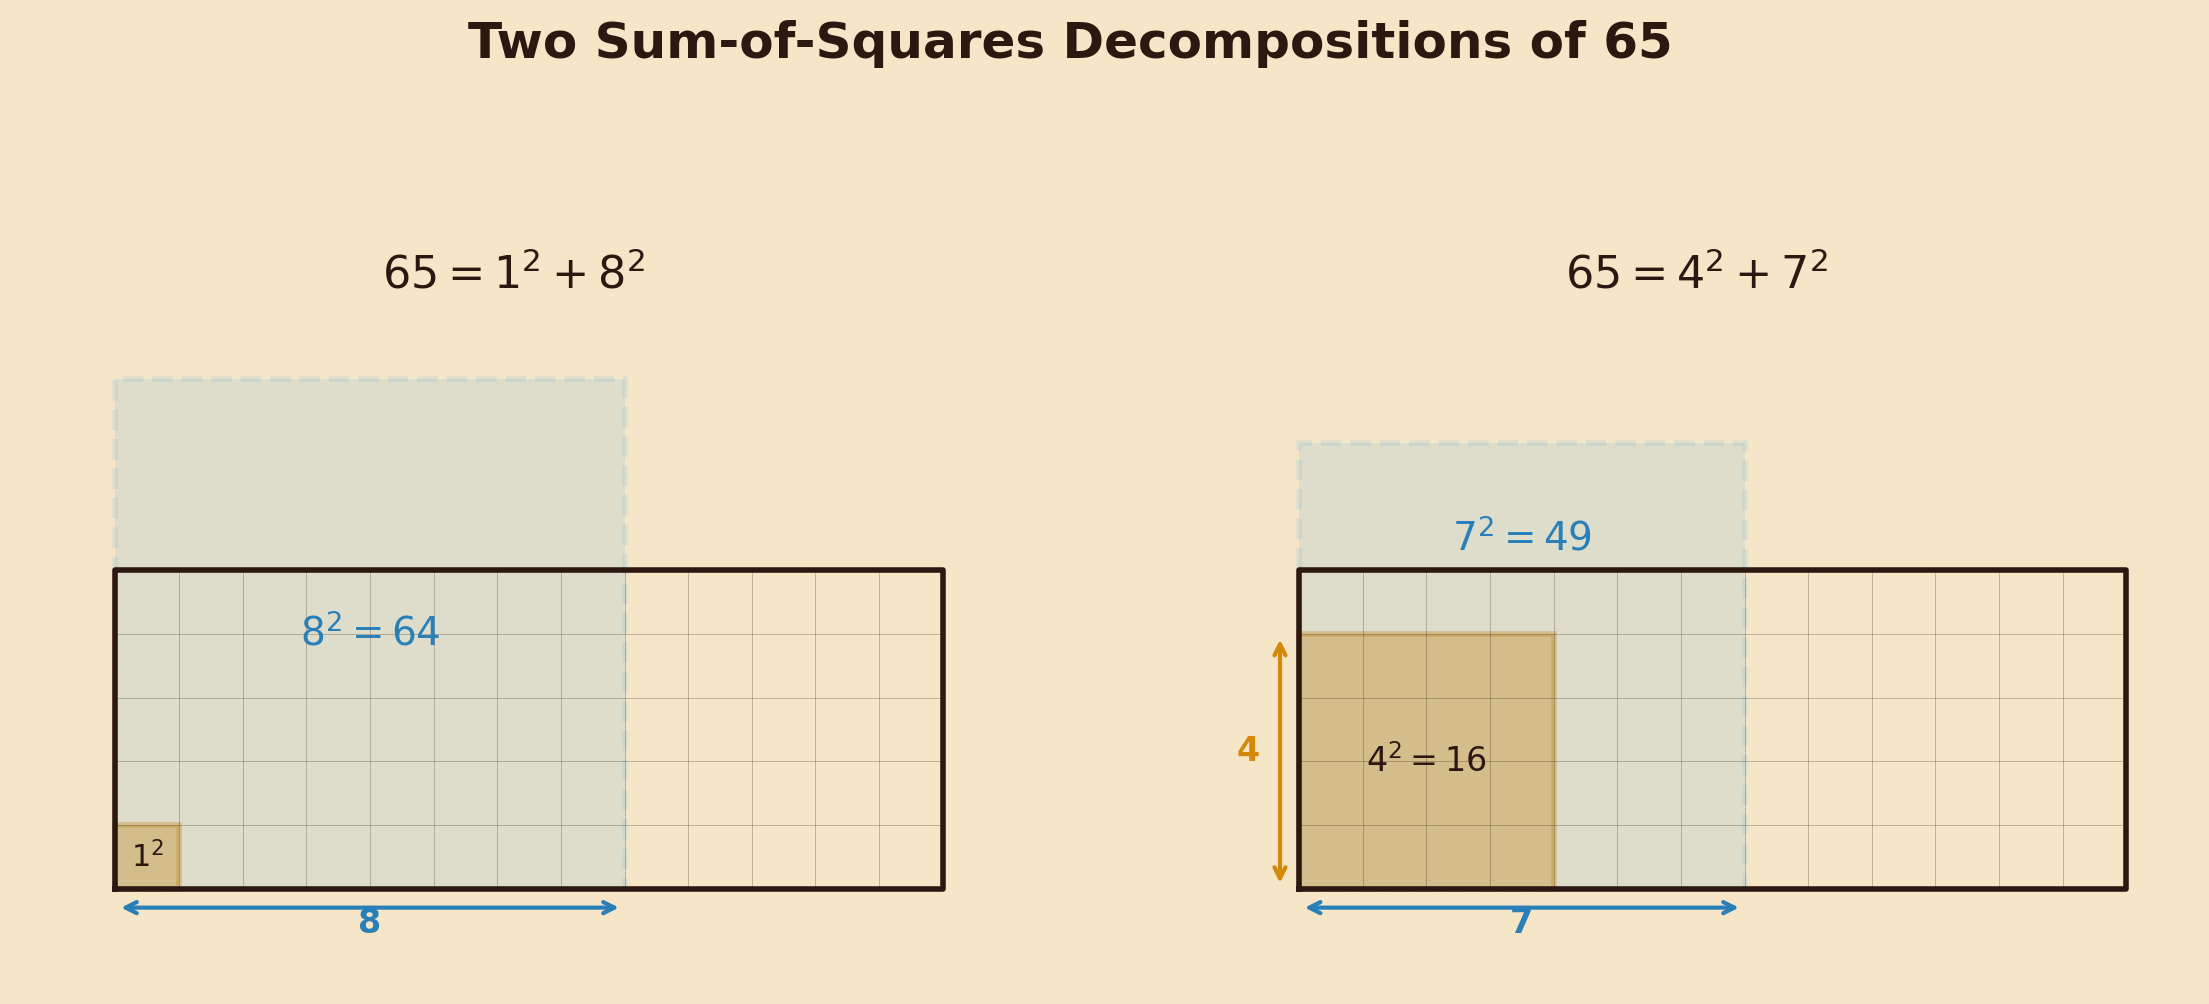
\includegraphics[width=0.85\textwidth]{Chapter4/images/fig01_rectangle_dissection.png}
\caption{}
\end{figure}
A \(13 \times 5\) rectangle subdivided into unit squares. Two different L-shaped dissections highlighted in contrasting colors (one in warm amber, the other in cool blue), each demonstrating a rearrangement into square-corner arrangements representing \(1^2 + 8^2\) and \(4^2 + 7^2\). The two dissections are shown side by side, with dotted lines indicating how one rearrangement of the same \(65\) unit squares produces two different sum-of-squares decompositions.{]}

The identity is called the \textbf{Brahmagupta--Fibonacci Identity}, and it has a pedigree that spans civilizations. Brahmagupta, the great Indian mathematician, stated a version of it in 628 AD in his \emph{Brāhmasphuṭasiddhānta} --- a monumental treatise on astronomy and arithmetic composed in the Sanskrit verse tradition. His interest was in what we now call Pell equations, but the multiplicative structure of sums of squares was a key ingredient. Nearly six centuries later, Fibonacci --- Leonardo of Pisa, the man who introduced Hindu-Arabic numerals to Europe --- rediscovered the identity in 1225 in his \emph{Liber Quadratorum}, a book devoted entirely to the theory of squares. Fibonacci likely learned it from Arabic sources, who in turn may have drawn on Indian mathematics. Ideas, like rivers, flow across borders.

But why does the identity work? The deepest explanation involves an idea that would not be formalized until the nineteenth century: \textbf{Gaussian integers}. Consider the complex number \(z_1 = a + bi\) and its companion \(z_2 = c + di\). The \emph{norm} of a Gaussian integer is the square of its absolute value: \(|z|^2 = z \cdot \bar{z}\). For \(z_1\), this is \(a^2 + b^2\); for \(z_2\), it is \(c^2 + d^2\). Now multiply:

\[z_1 \cdot z_2 = (a + bi)(c + di) = (ac - bd) + (ad + bc)i.\]

The norm of this product is \((ac - bd)^2 + (ad + bc)^2\). But the fundamental law of norms says \(|z_1 z_2|^2 = |z_1|^2 \cdot |z_2|^2\). And there it is --- the Brahmagupta--Fibonacci identity is simply the statement that \emph{the norm of a product equals the product of the norms}. The algebra of complex multiplication is doing all the work behind the curtain.


\begin{figure}[htbp]
\centering
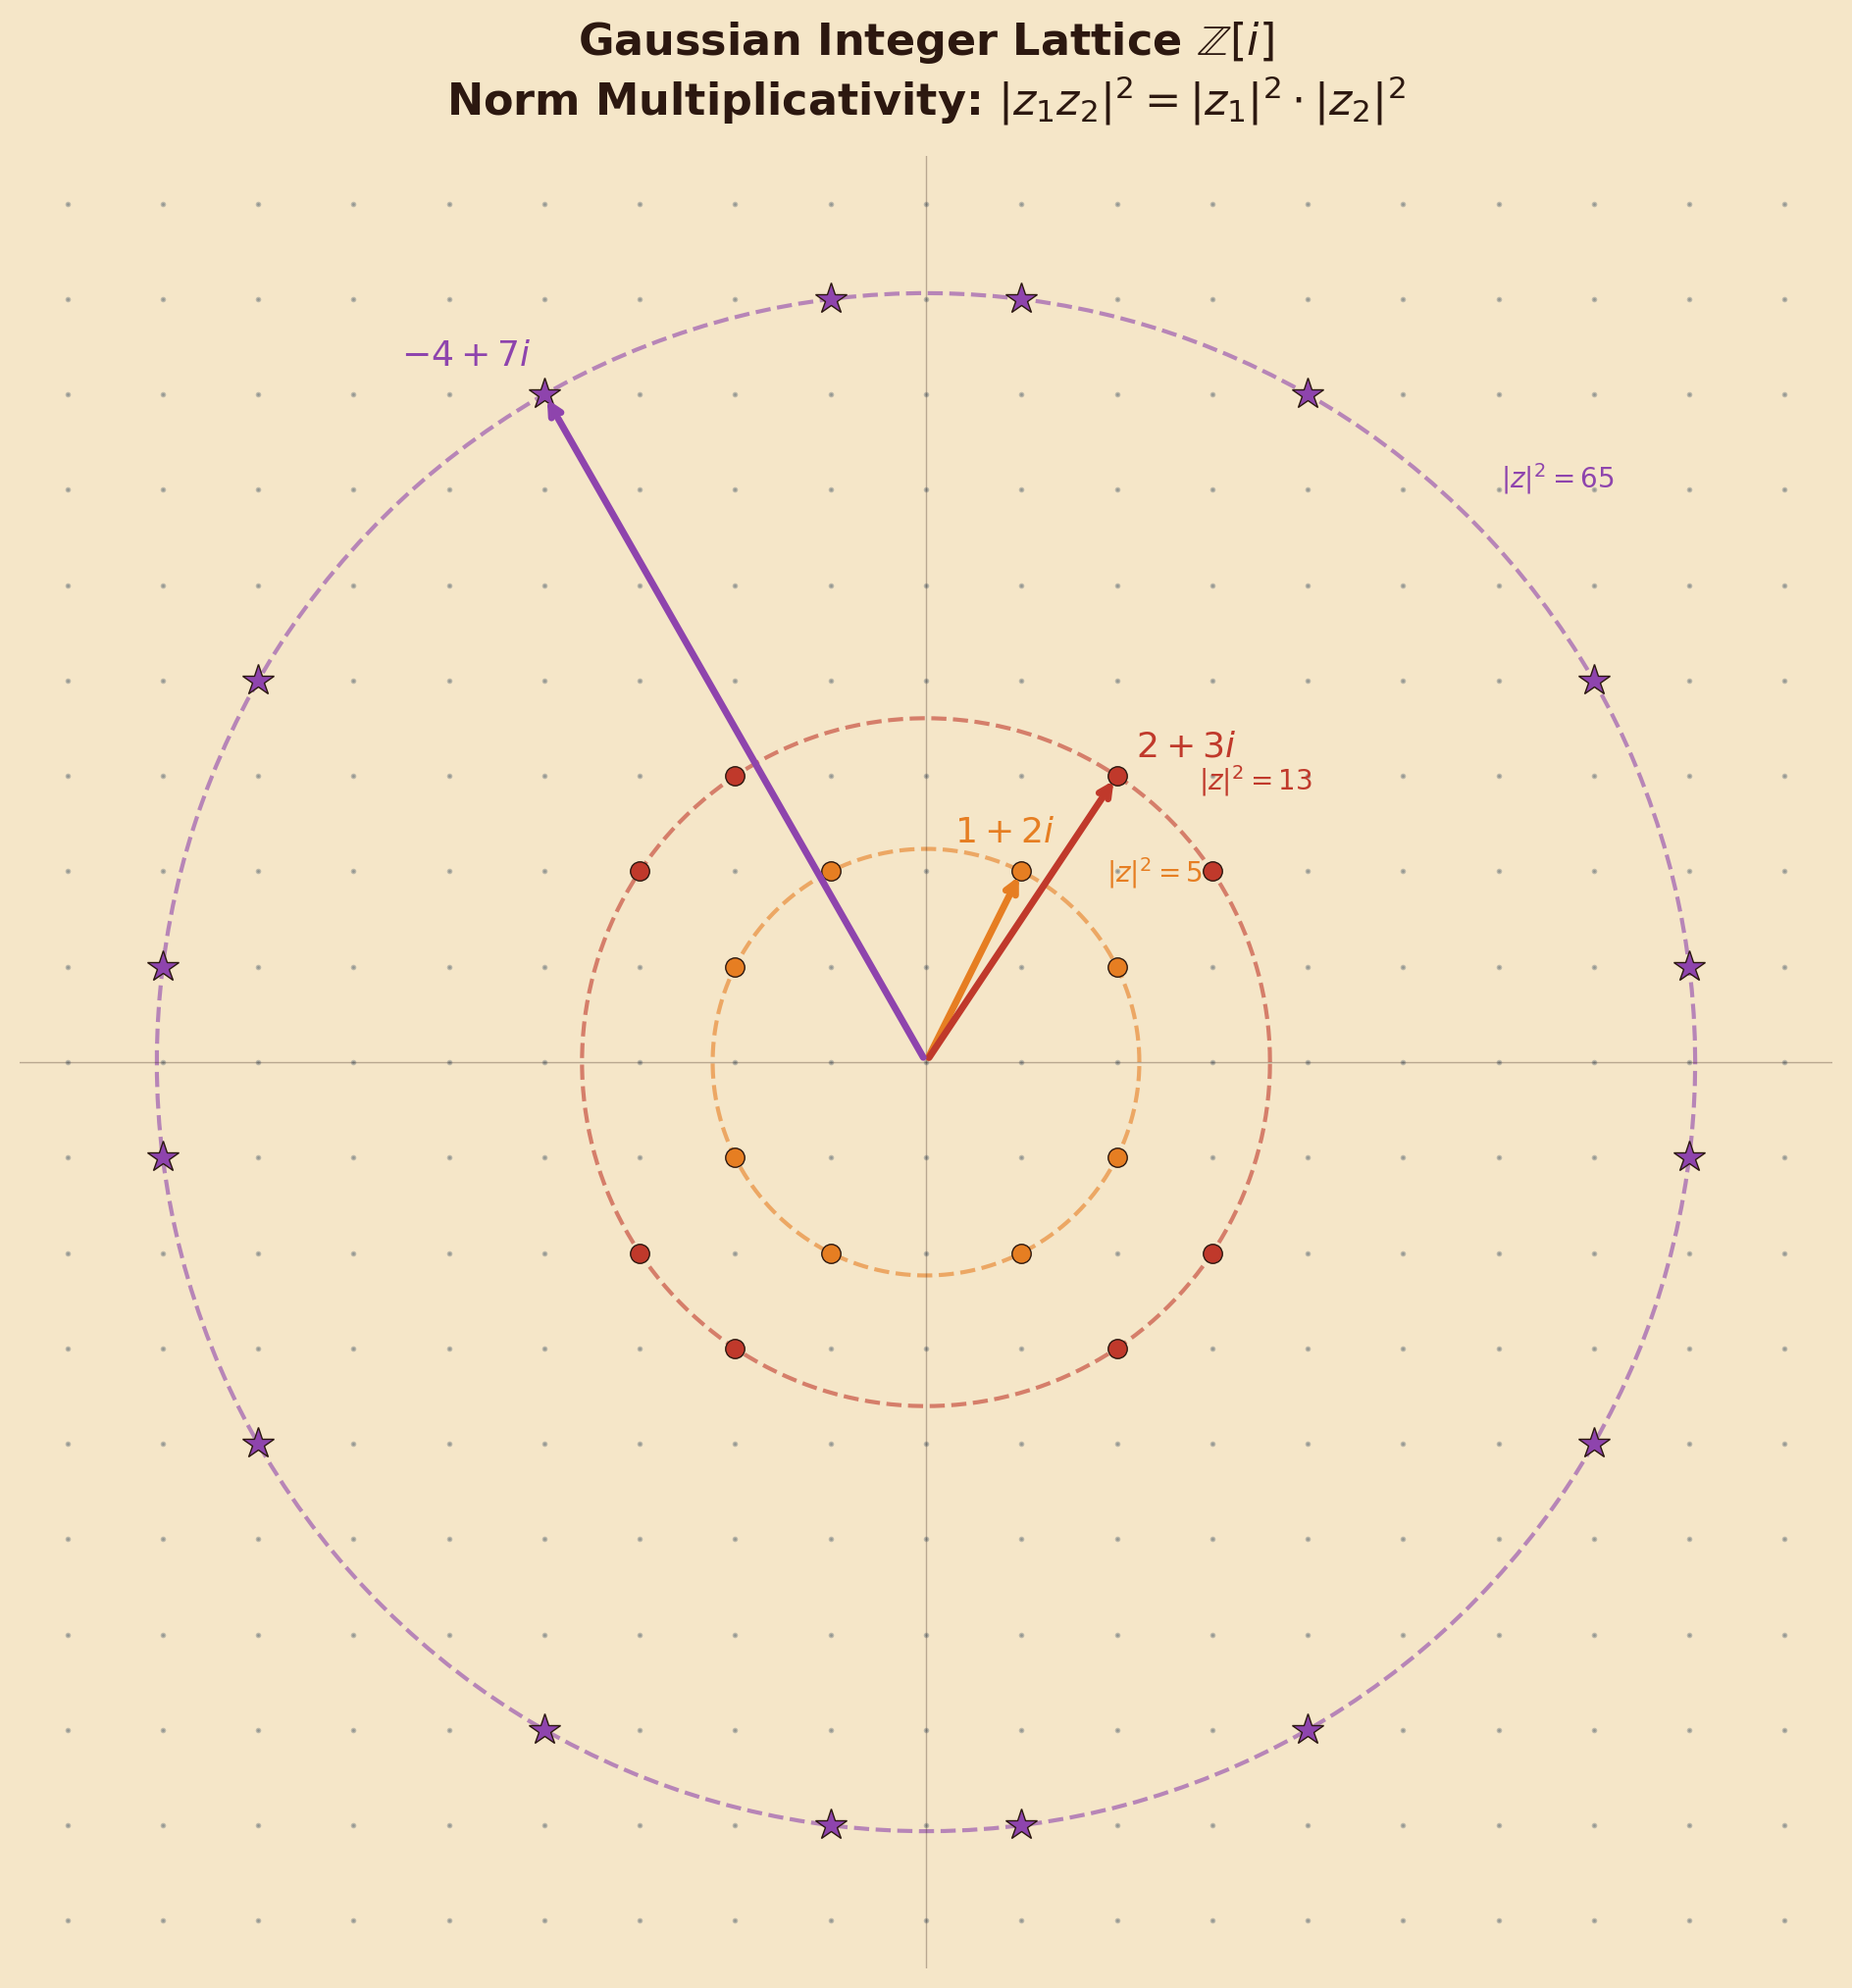
\includegraphics[width=0.85\textwidth]{Chapter4/images/fig02_gaussian_lattice.png}
\caption{}
\end{figure}
The Gaussian integer lattice \(\mathbb{Z}[i]\) in the complex plane. Points \(1+2i\) and \(2+3i\) are shown as vectors from the origin, drawn in contrasting colors. Their product \(-4+7i\) is shown as a third vector. Three concentric circles centered at the origin pass through lattice points: \(|z|^2 = 5\) (through \(1+2i\) and \(2+i\)), \(|z|^2 = 13\) (through \(2+3i\) and \(3+2i\)), and \(|z|^2 = 65\) (through \(-4+7i\), \(4+7i\), \(1+8i\), \(8+i\), and their reflections). The two factorizations of \(65\) correspond to two distinct lattice points on the outermost circle, highlighted with small starbursts.{]}

The Gaussian integers transform the Brahmagupta--Fibonacci identity from a clever algebraic trick into an inevitable consequence of how multiplication works in the complex plane. Every time you multiply two numbers that are sums of two squares, the product is \emph{automatically} a sum of two squares --- and typically in more than one way, because you can conjugate one factor before multiplying (\(z_1 \cdot \bar{z}_2\) instead of \(z_1 \cdot z_2\)) and get a different decomposition. The two representations of \(65\) are not a coincidence; they are reflections of two different paths through the Gaussian lattice to the same destination.

\bigskip\noindent\rule{\linewidth}{0.4pt}\bigskip

\section{A Factory for Pythagorean Triples}
Now watch how the curtain rises on a larger stage.

Hand me any two Pythagorean triples. I don't care which ones --- pick your favorites. I will combine them to produce a \emph{new} Pythagorean triple whose hypotenuse is the product of the two original hypotenuses. Every time, without fail.

Let's try it. Take \((3, 4, 5)\) and \((5, 12, 13)\). The first triple says \(3^2 + 4^2 = 5^2\); the second says \(5^2 + 12^2 = 13^2\). I claim there is a Pythagorean triple with hypotenuse \(5 \times 13 = 65\). And the Brahmagupta--Fibonacci identity hands it to us:

\[(3 \cdot 5 - 4 \cdot 12)^2 + (3 \cdot 12 + 4 \cdot 5)^2 = (15 - 48)^2 + (36 + 20)^2 = (-33)^2 + 56^2 = 1089 + 3136 = 4225 = 65^2.\]

So \((33, 56, 65)\) is a Pythagorean triple. The second variant of the identity gives us another:

\[(3 \cdot 5 + 4 \cdot 12)^2 + (3 \cdot 12 - 4 \cdot 5)^2 = 63^2 + 16^2 = 3969 + 256 = 4225 = 65^2.\]

And \((16, 63, 65)\) is also Pythagorean. Two triples in, two new triples out --- a factory running on pure algebra.


\begin{figure}[htbp]
\centering
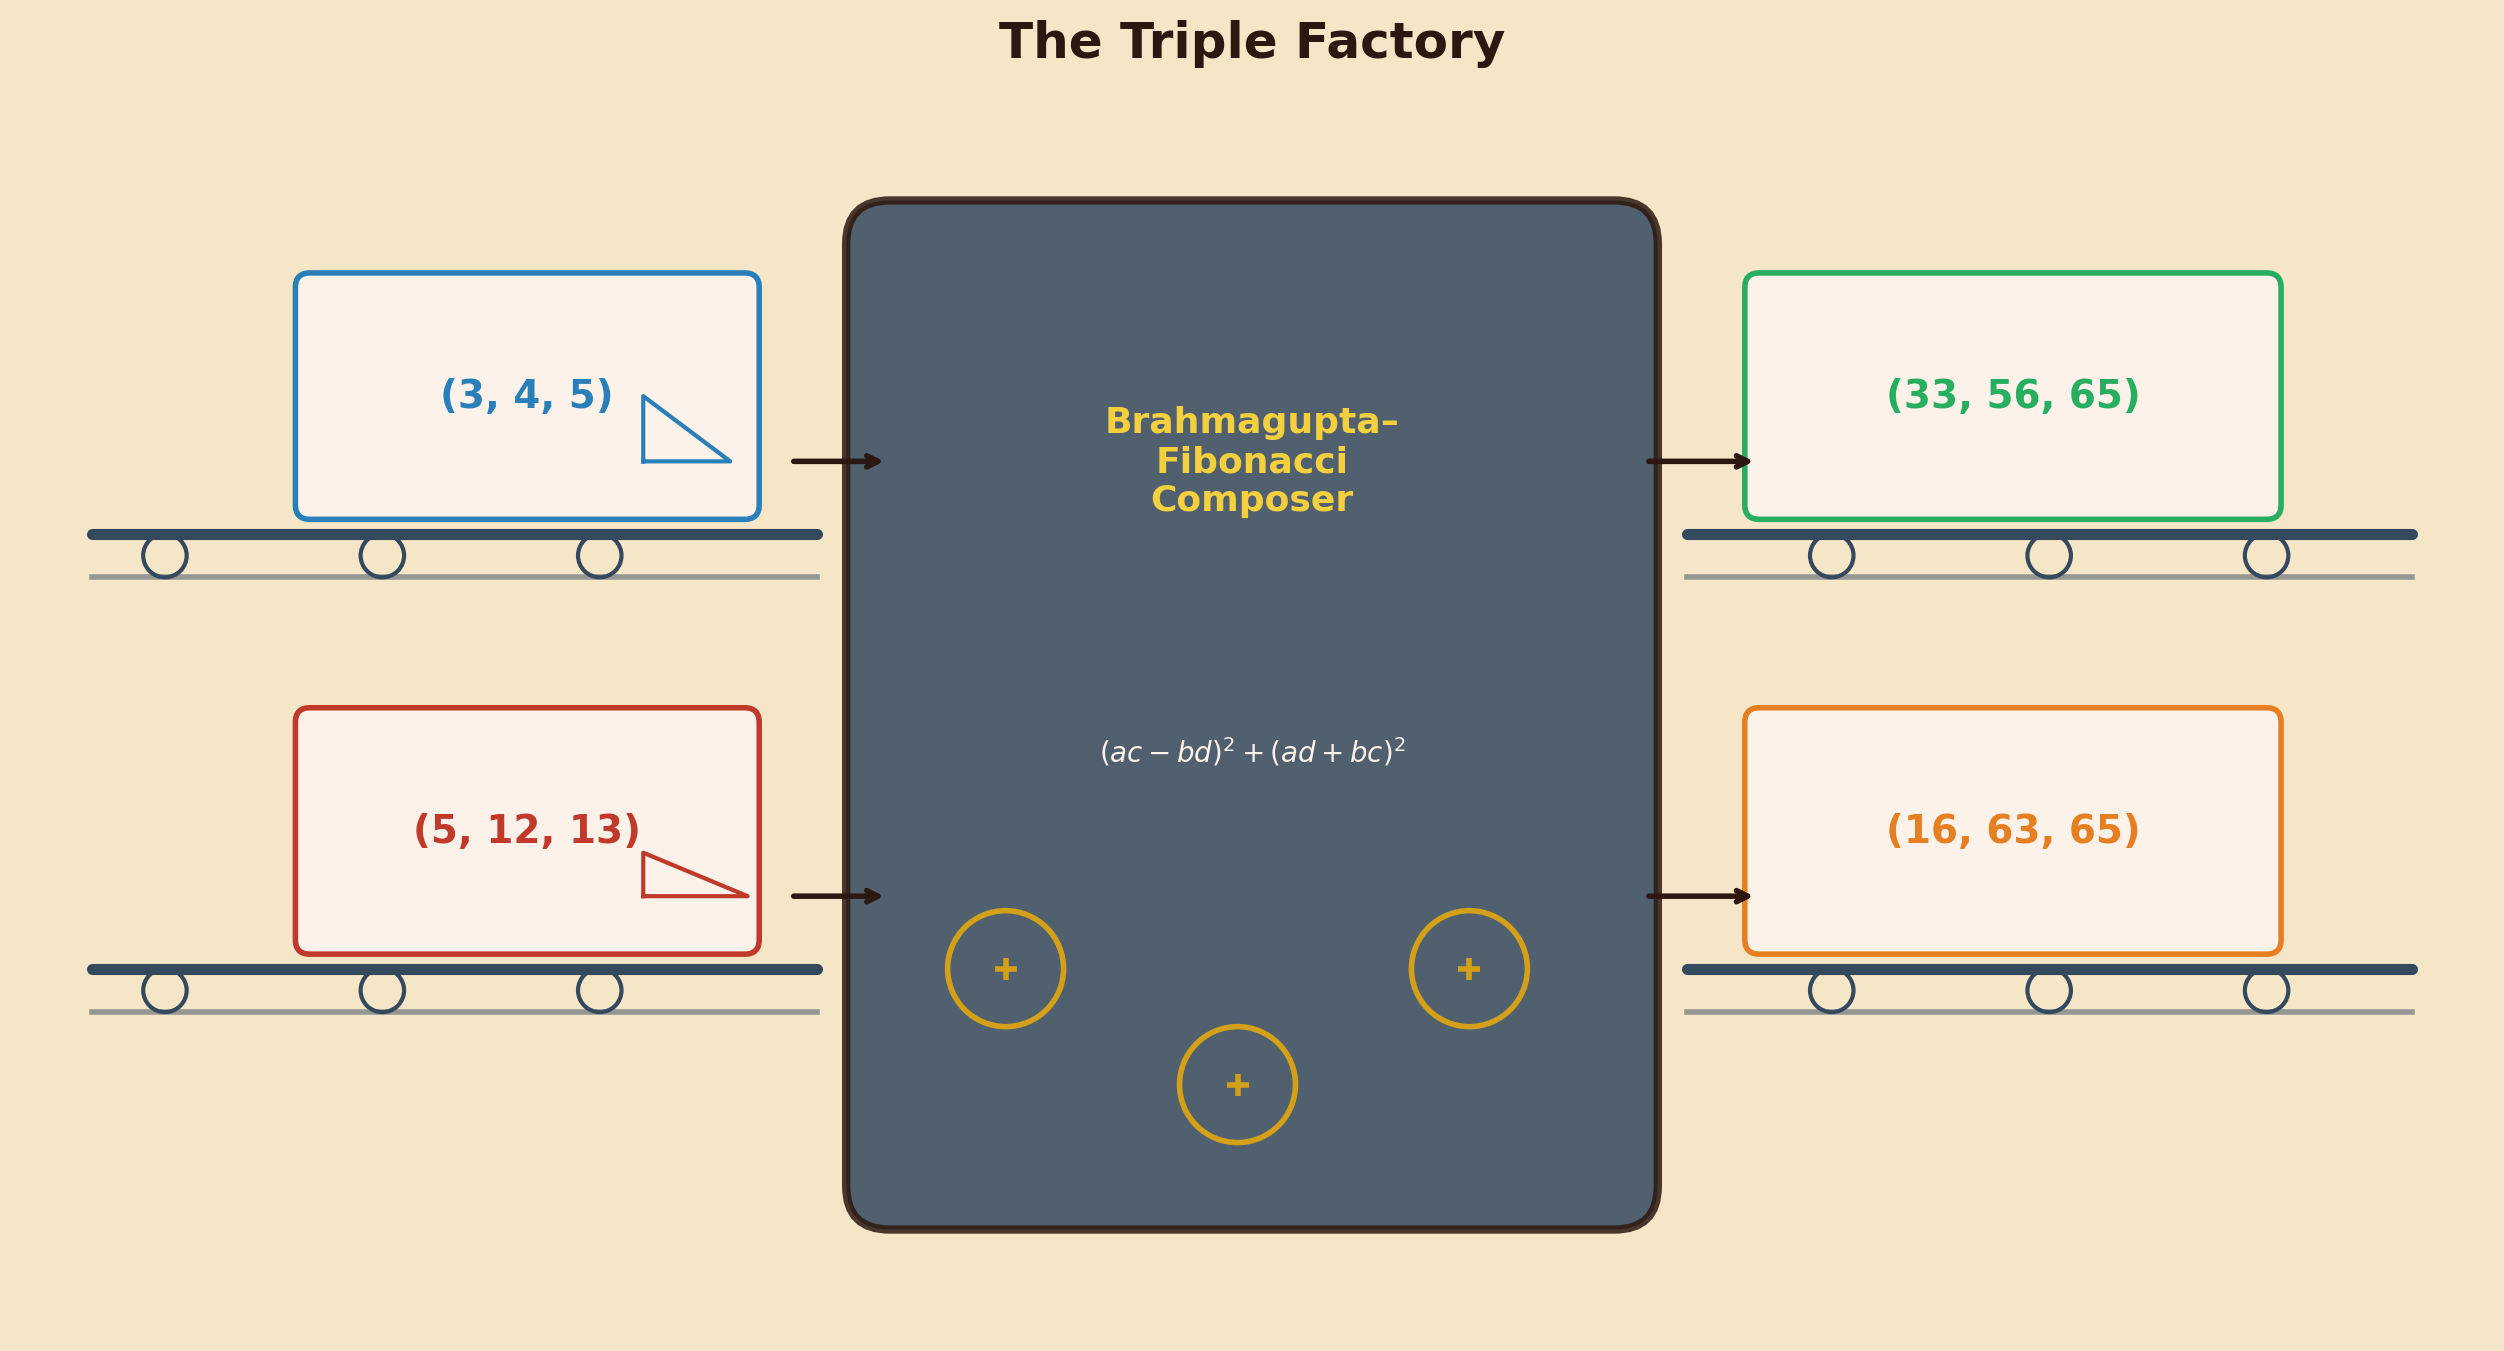
\includegraphics[width=0.85\textwidth]{Chapter4/images/fig03_triple_factory.png}
\caption{}
\end{figure}
A whimsical ``Triple Factory'' conveyor belt diagram. Two input conveyor belts enter from the left, one carrying a card labeled \((3, 4, 5)\) with a small right triangle drawn on it, the other carrying \((5, 12, 13)\) with its right triangle. Both belts feed into a central machine labeled ``Brahmagupta--Fibonacci Composer'' adorned with gears and the identity formula. Two output belts emerge on the right, one carrying \((33, 56, 65)\) and the other \((16, 63, 65)\). Below each card, the corresponding right triangle is drawn to scale, showing how the output triangles are larger.{]}

Let us state this precisely.

\textbf{Pythagorean Composition Theorem.} If \(a_1^2 + b_1^2 = c_1^2\) and \(a_2^2 + b_2^2 = c_2^2\), then

\[(a_1 a_2 - b_1 b_2)^2 + (a_1 b_2 + b_1 a_2)^2 = (c_1 c_2)^2.\]

\emph{Proof.} The left side is \((a_1^2 + b_1^2)(a_2^2 + b_2^2)\) by the Brahmagupta--Fibonacci identity. But \(a_1^2 + b_1^2 = c_1^2\) and \(a_2^2 + b_2^2 = c_2^2\), so this equals \(c_1^2 \cdot c_2^2 = (c_1 c_2)^2\). \(\square\)

The elegance here is almost unreasonable. The composition of Pythagorean triples is not some ad hoc construction --- it is multiplication of Gaussian integers in disguise. The triple \((a, b, c)\) corresponds to the Gaussian integer \(a + bi\) with norm \(c\). Composing two triples is just multiplying the corresponding Gaussian integers and reading off the new legs from the real and imaginary parts. Gauss understood this in the early 1800s, and it led him to one of the most beautiful theorems in number theory: a prime \(p\) can be written as the sum of two squares if and only if \(p = 2\) or \(p \equiv 1 \pmod{4}\).


\begin{figure}[htbp]
\centering
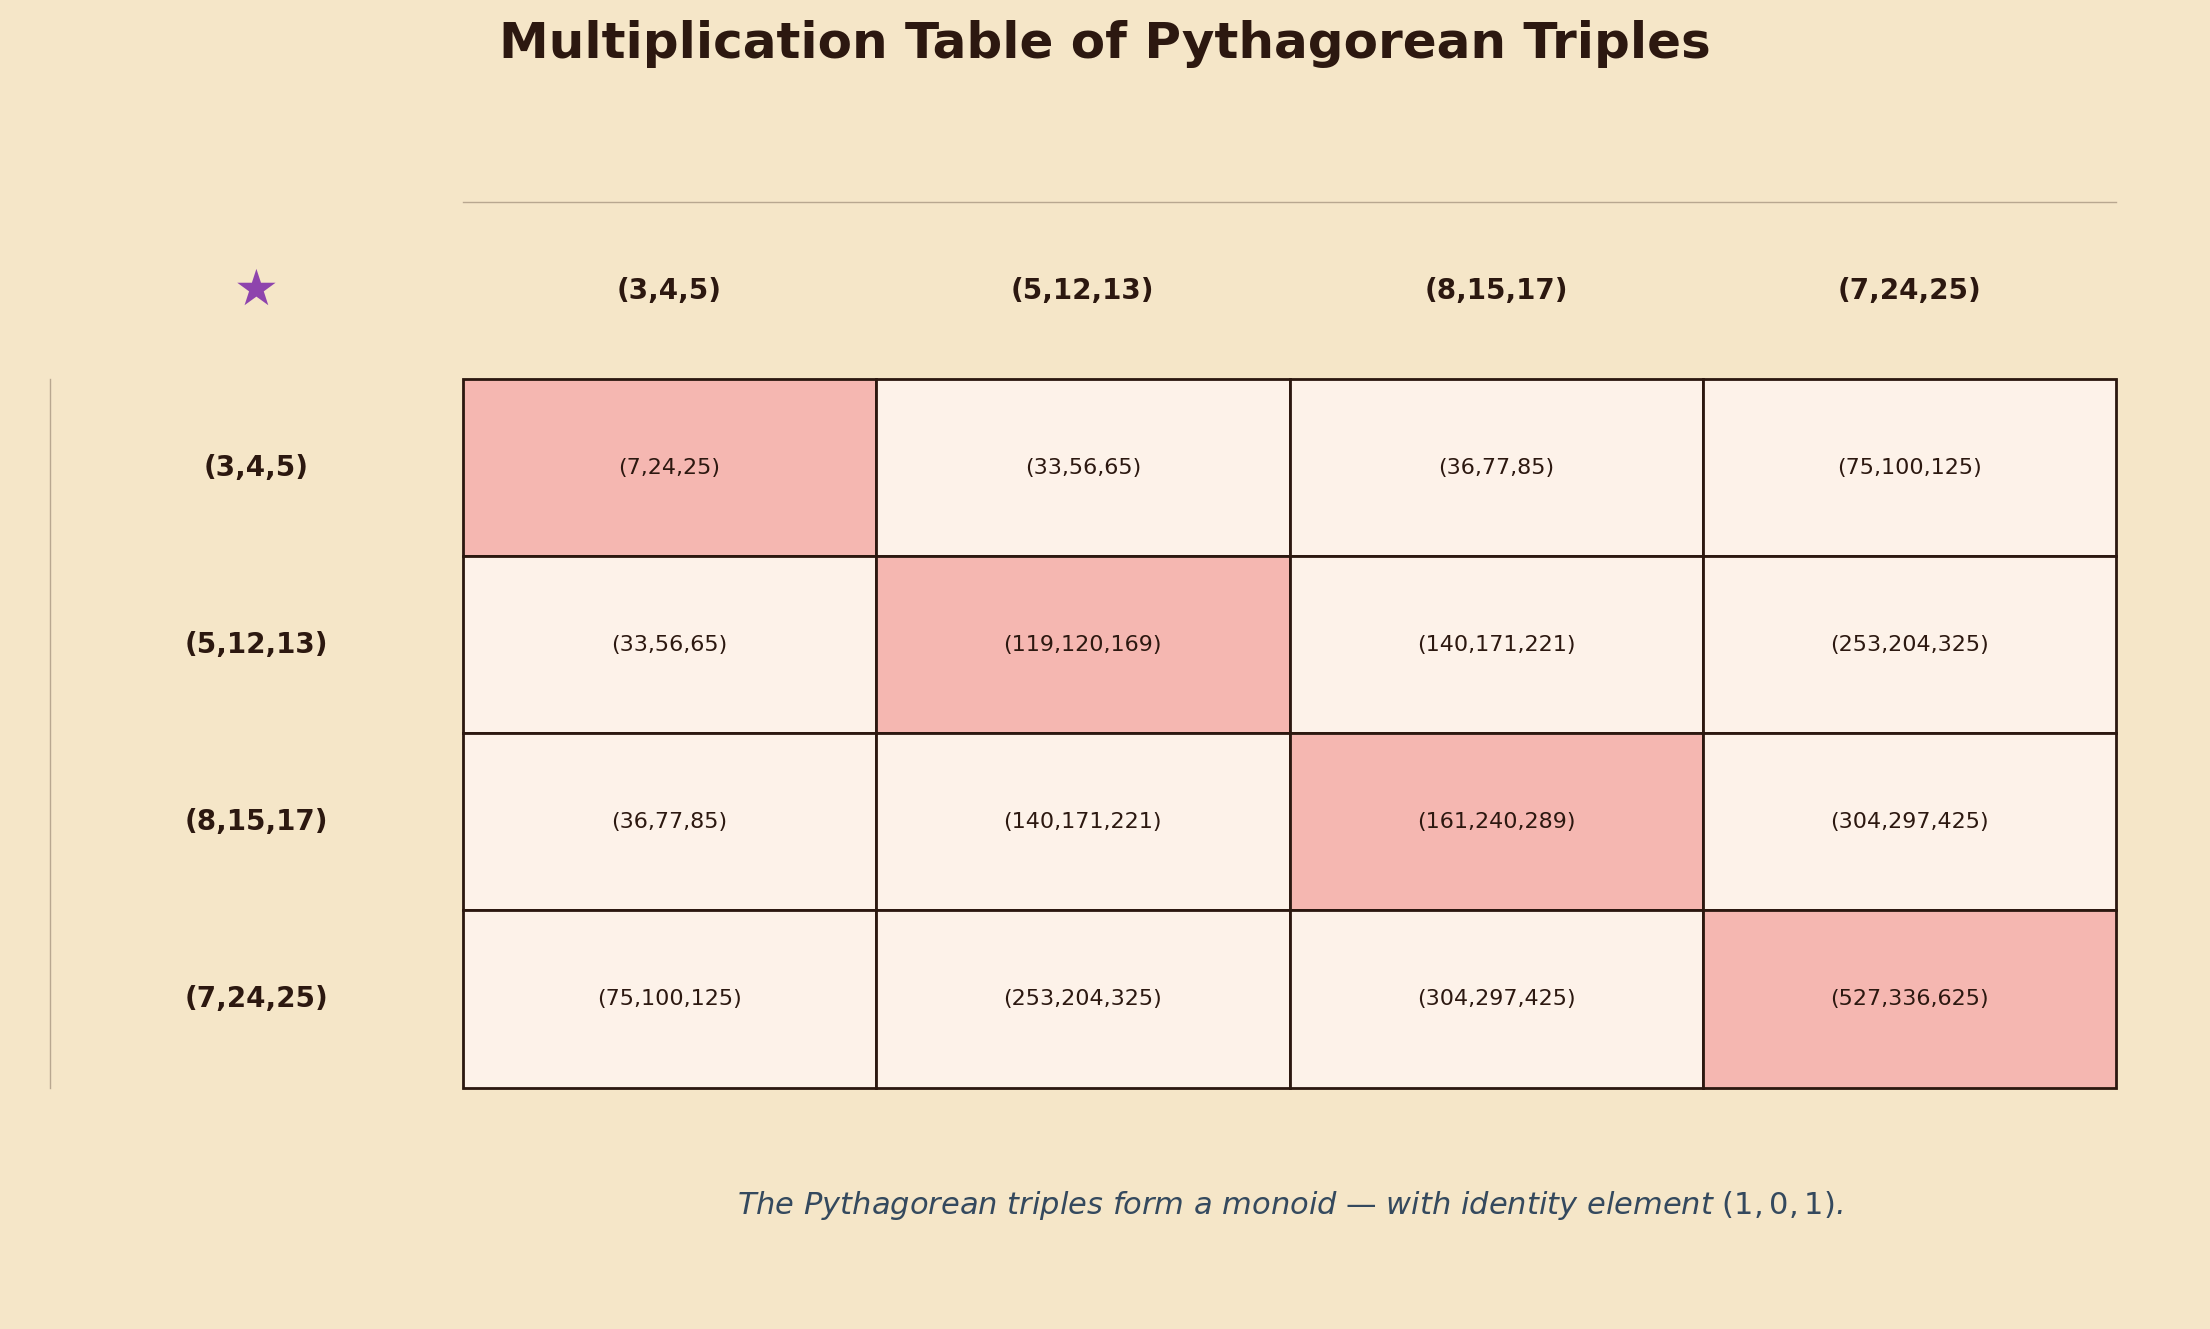
\includegraphics[width=0.85\textwidth]{Chapter4/images/fig04_multiplication_table.png}
\caption{}
\end{figure}
A multiplication table of small Pythagorean triples. Rows and columns are headed by \((3,4,5)\), \((5,12,13)\), \((8,15,17)\), and \((7,24,25)\). Each cell shows the composed triple (using the first variant of the identity). The diagonal entries --- a triple composed with itself --- are highlighted, showing ``squares'' like \((3,4,5) \star (3,4,5) = (-7, 24, 25)\), which after taking absolute values gives \((7, 24, 25)\). A note below the table reads: ``The Pythagorean triples form a monoid --- a set with an associative binary operation and an identity element \((1, 0, 1)\).''{]}

The word \emph{monoid} deserves a moment's attention for those who have not met it. A monoid is simply a collection of objects equipped with a way of combining any two of them to get a third, where the operation is associative and there is an identity element that does nothing. The integers under addition form a monoid (with identity \(0\)). The Pythagorean triples under Brahmagupta--Fibonacci composition form a monoid too, with identity \((1, 0, 1)\) --- the degenerate ``triple'' where one leg vanishes. Compose any triple with \((1, 0, 1)\) and you get the same triple back, just as adding \(0\) to a number leaves it unchanged. The Pythagorean triples are not merely a list; they are a \emph{structure}.

\bigskip\noindent\rule{\linewidth}{0.4pt}\bigskip

\section{Euler's Jewel --- Cracking Numbers with Two Portraits}
We have seen that multiplying sums of squares gives new sums of squares, often in more than one way. Now I want to show you how this multiplicity of representations can be turned into a \emph{weapon} --- a tool for cracking numbers apart.

If a number \(N\) confesses its identity as a sum of two squares in \emph{two different ways}, it is giving away its factors.

This observation belongs to Euler, who spent decades wrestling with the arithmetic of sums of squares. His correspondence with Goldbach, stretching from 1730 to 1764, is one of the great mathematical dialogues of the eighteenth century, and sums of squares were a recurring theme. Fermat had claimed, without proof, that every prime of the form \(4k + 1\) is a sum of two squares. Euler was determined to prove it --- and along the way, he discovered a factoring method of surprising beauty.

Here is how it works. Suppose you know that

\[N = a^2 + b^2 = c^2 + d^2\]

with the two representations \emph{essentially different} --- meaning it's not just a matter of swapping the order of the squares or flipping signs. Then:

\[(a^2 - c^2) = (d^2 - b^2),\]

which we can factor as:

\[(a - c)(a + c) = (d - b)(d + b).\]

Now compute \(\gcd(a - c, d - b)\) and \(\gcd(a + c, d + b)\). With a bit of careful arithmetic, at least one of these GCDs will share a non-trivial common factor with \(N\), splitting it open.


\begin{figure}[htbp]
\centering
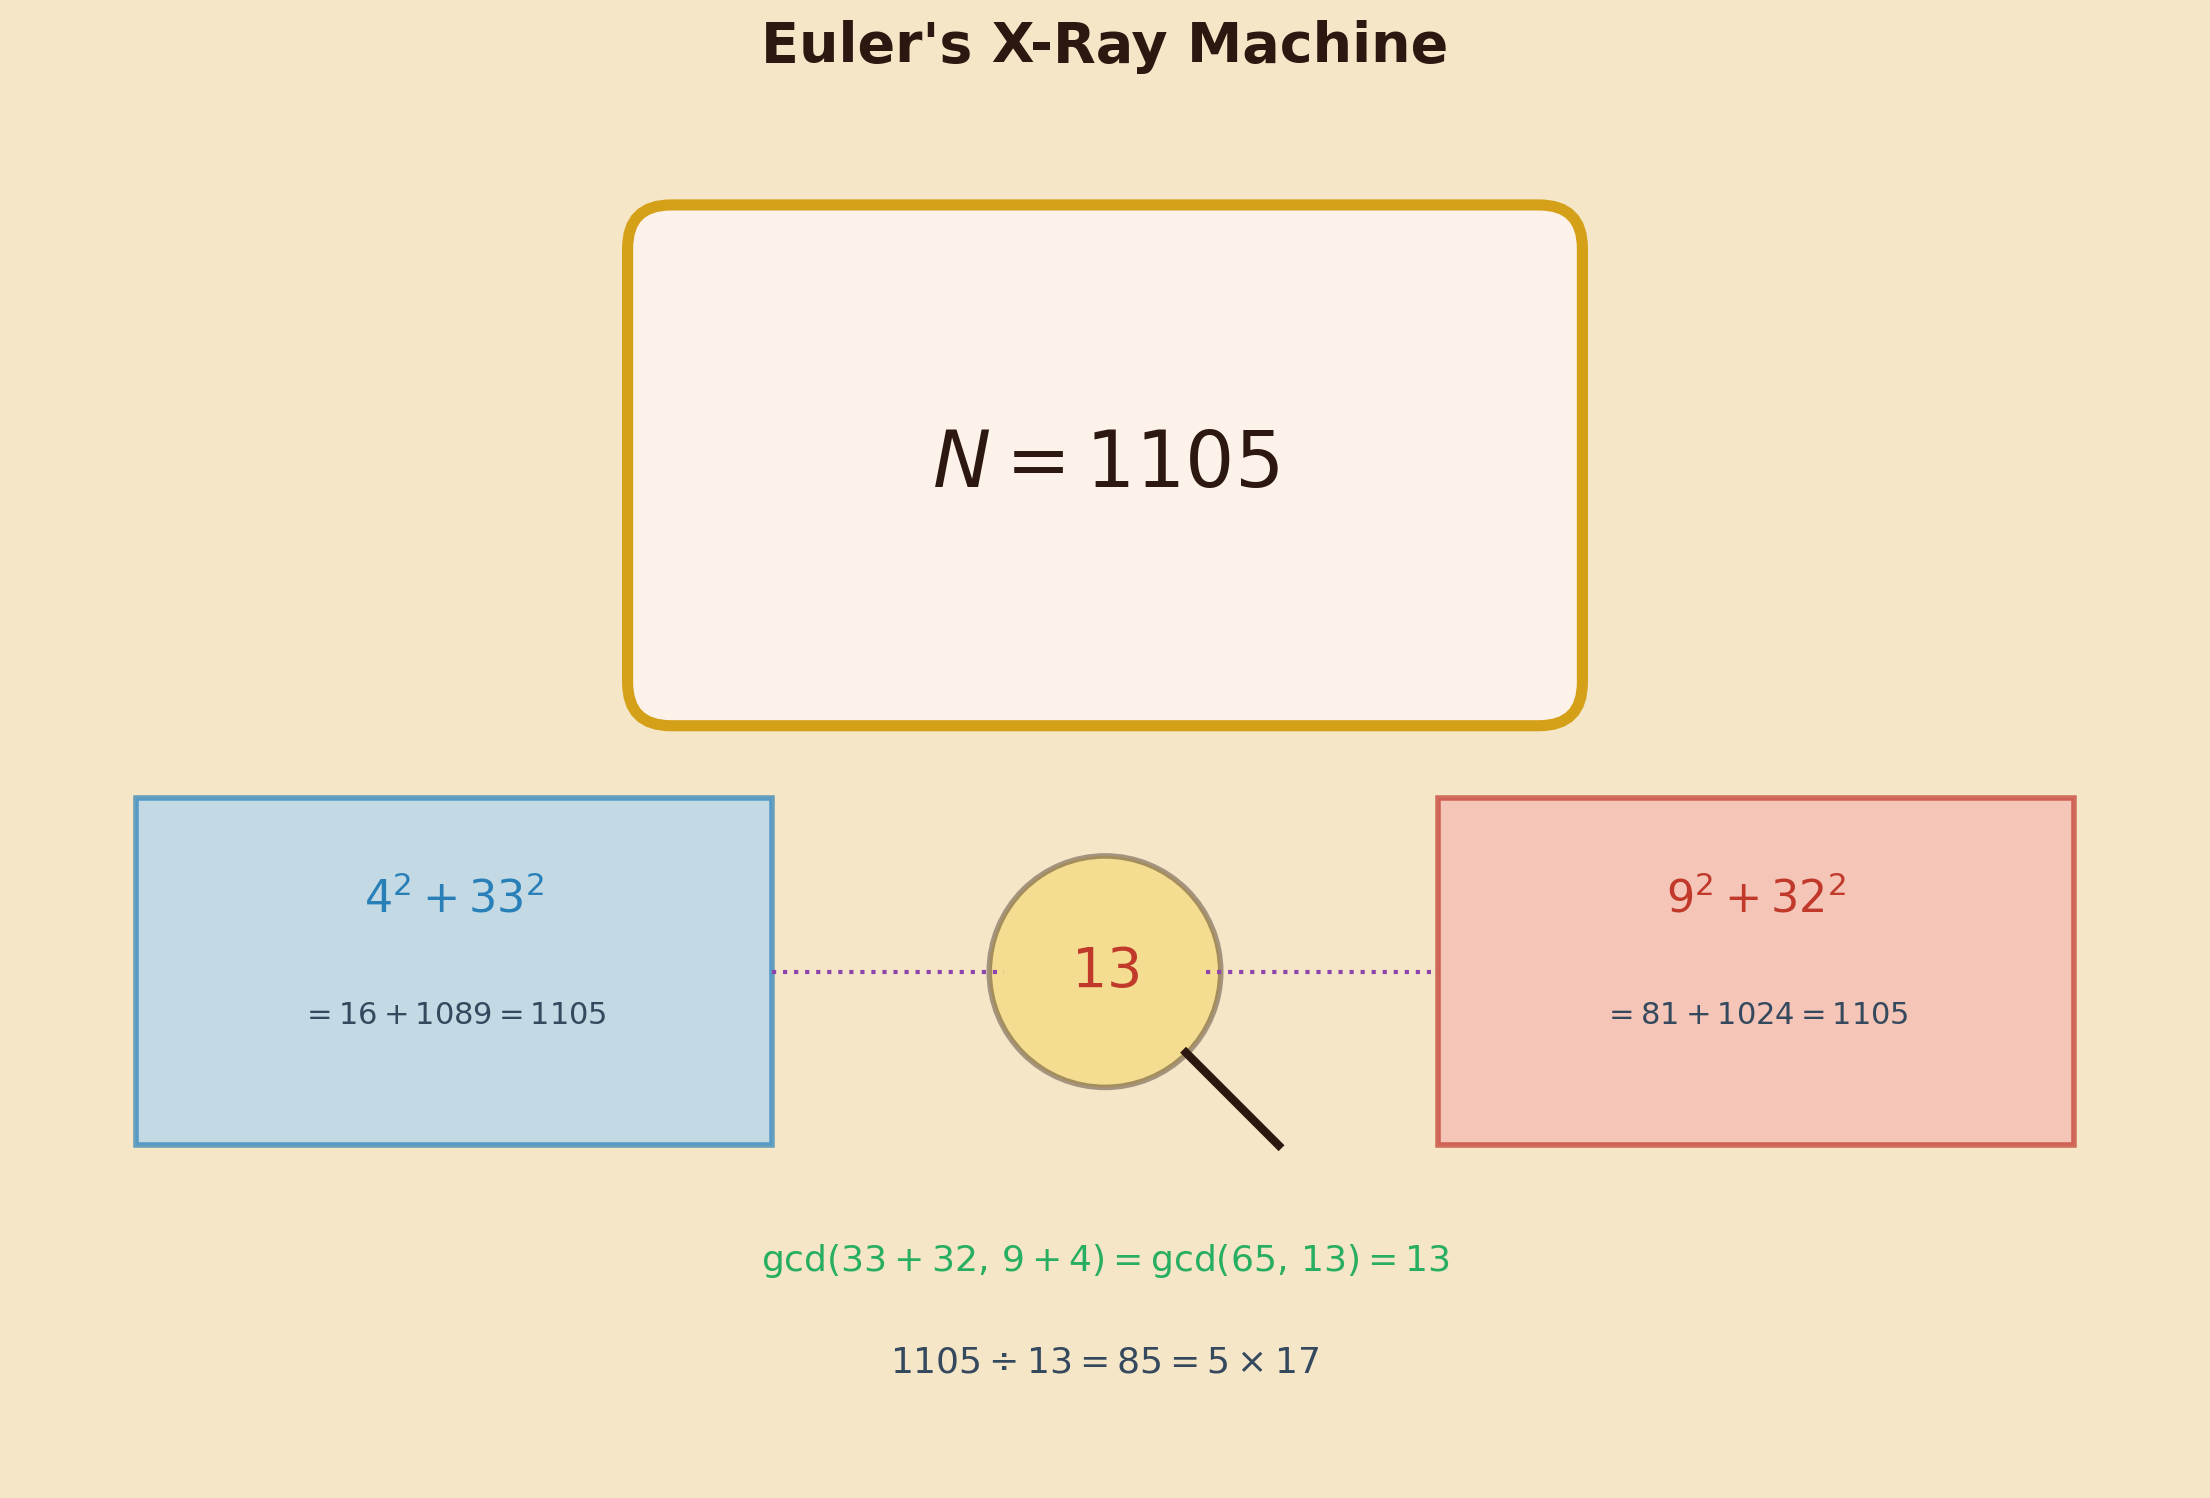
\includegraphics[width=0.85\textwidth]{Chapter4/images/fig05_euler_xray.png}
\caption{}
\end{figure}
``Euler's X-Ray Machine.'' A large number \(N = 1105\) sits inside an ornate picture frame. On either side, two X-ray screens display the number's inner structure: the left screen shows \(4^2 + 33^2 = 16 + 1089 = 1105\), and the right screen shows \(9^2 + 32^2 = 81 + 1024 = 1105\). Dotted lines connect corresponding terms across the two screens, crossing at a magnifying glass in the center. Through the magnifying glass, the factor \(13\) is visible, glowing. Below the frame, the arithmetic: \(\gcd(33 - 32, 9 - 4) = \gcd(1, 5) = 1\) --- no luck. But \(\gcd(33 + 32, 9 + 4) = \gcd(65, 13) = 13\) --- and \(1105 / 13 = 85 = 5 \times 17\).{]}

Let us walk through the example. Take \(N = 1105\). A little experimentation reveals two representations:

\[1105 = 4^2 + 33^2 = 9^2 + 32^2.\]

So \(a = 33\), \(b = 4\), \(c = 32\), \(d = 9\) (rearranging so \(a > b\) and \(c > d\)). Compute:

\[a - c = 33 - 32 = 1, \quad a + c = 33 + 32 = 65,\] \[d - b = 9 - 4 = 5, \quad d + b = 9 + 4 = 13.\]

Now: \(\gcd(65, 1105) = 65\)? Let's check: \(1105 / 65 = 17\). So \(1105 = 65 \times 17\). And \(65 = 5 \times 13\), so:

\[1105 = 5 \times 13 \times 17.\]

From two sum-of-squares representations, we extracted the complete factorization. Euler had essentially built an X-ray machine for composite numbers: shine two different ``portraits'' of \(N\) at each other, and the interference pattern reveals the hidden structure.


\begin{figure}[htbp]
\centering
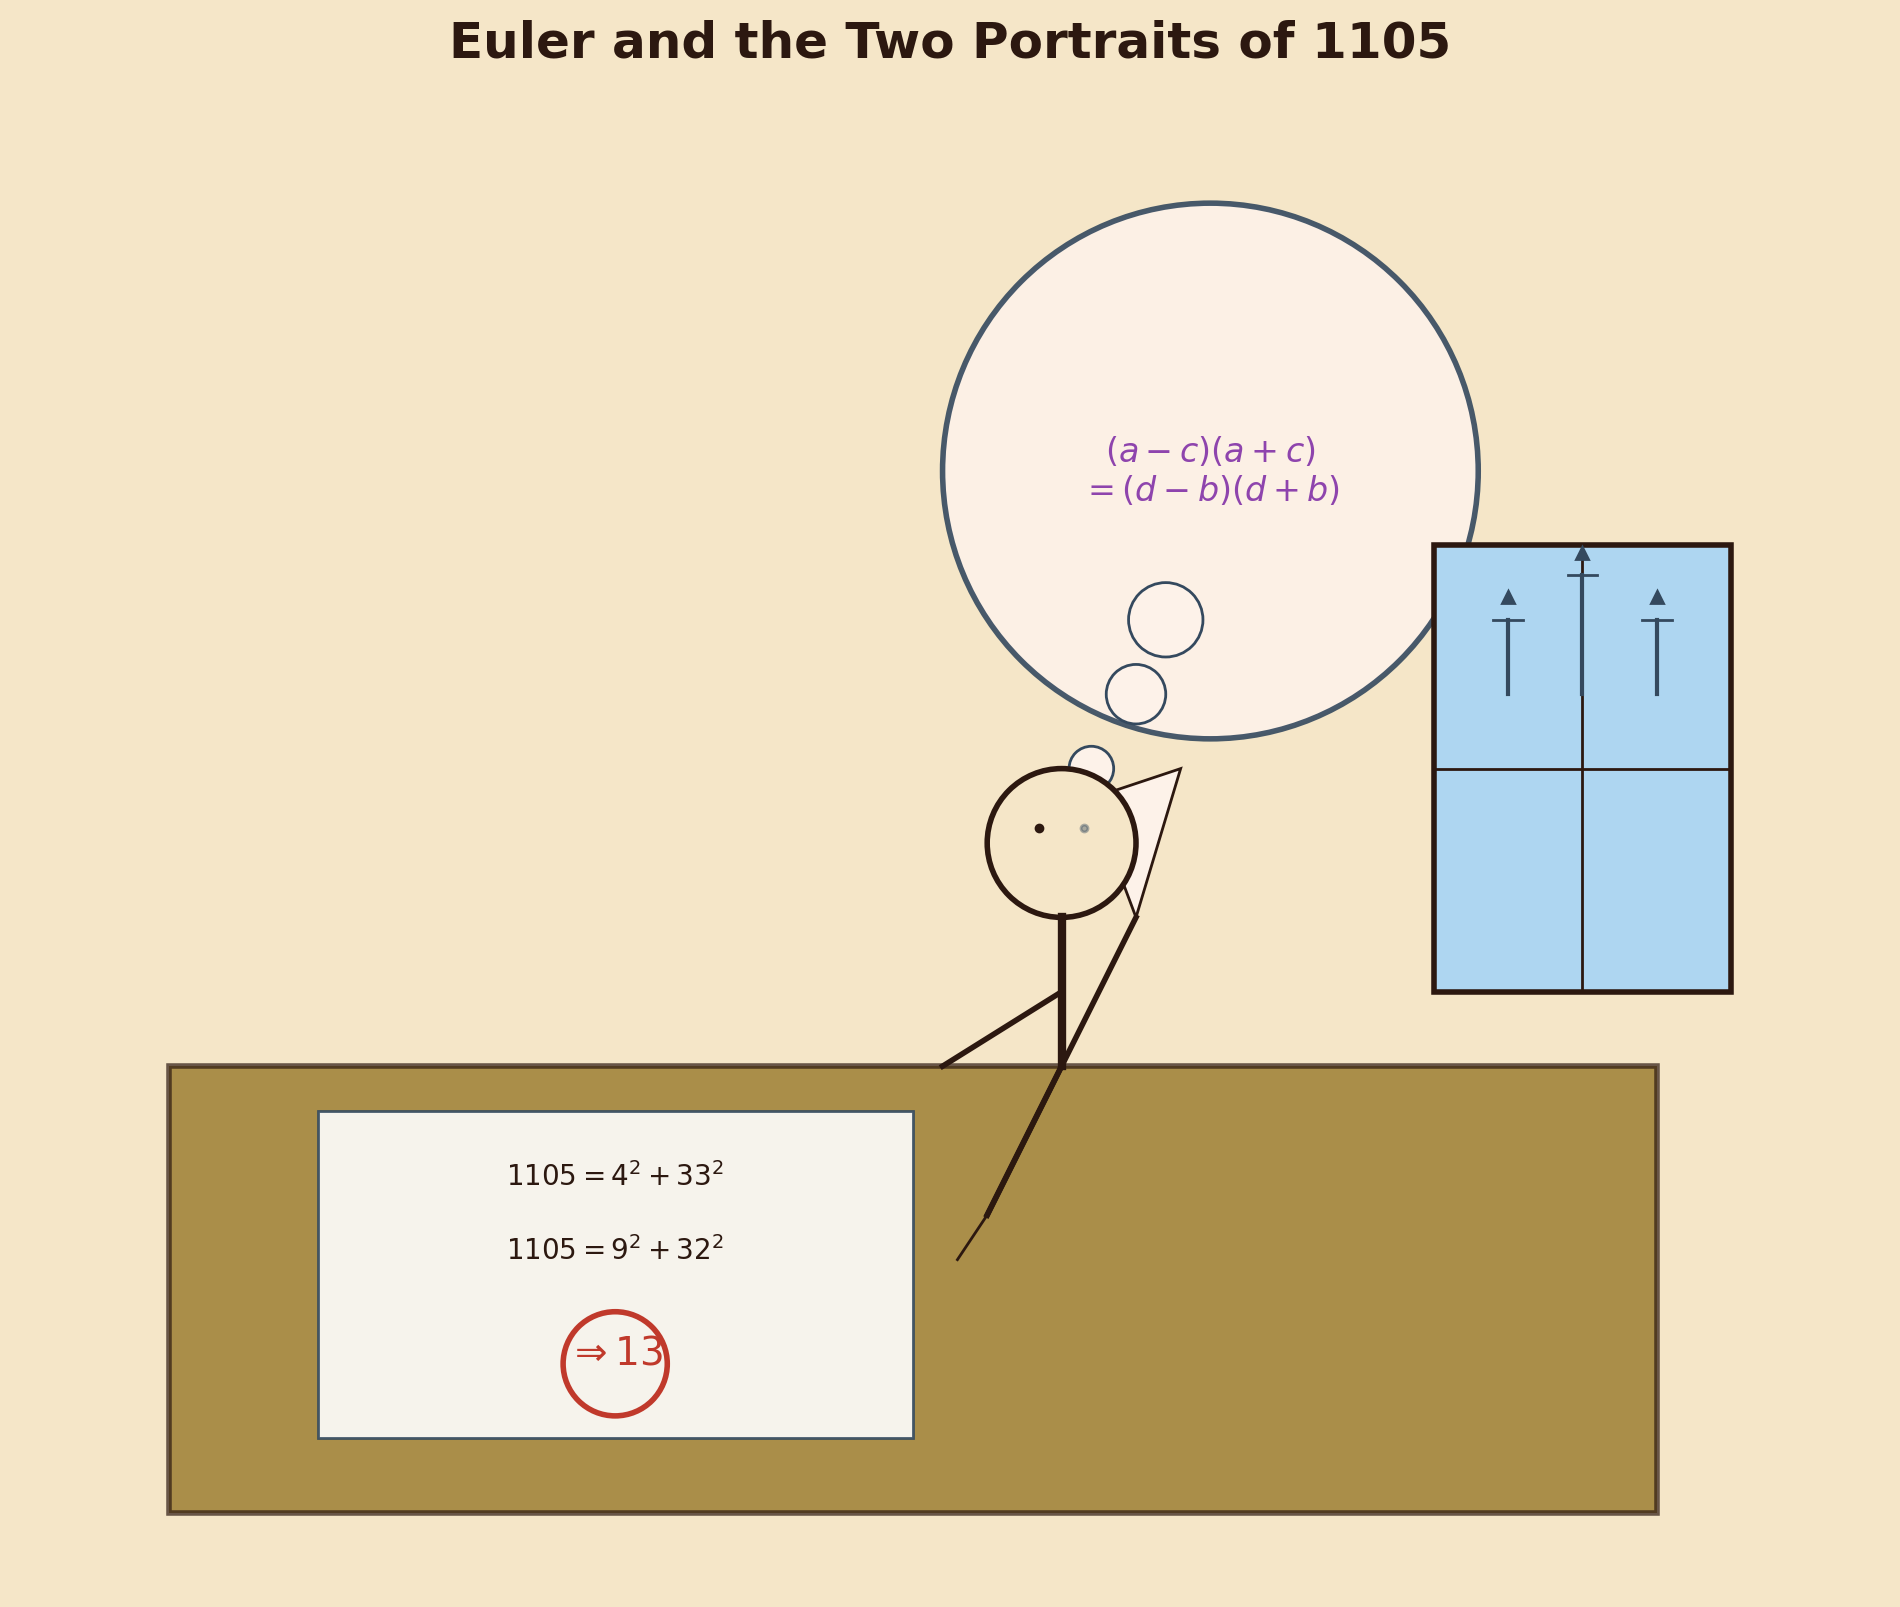
\includegraphics[width=0.85\textwidth]{Chapter4/images/fig06_euler_portrait.png}
\caption{}
\end{figure}
A portrait sketch of Leonhard Euler at his desk, quill in hand, late in life (one eye clouded over). A thought bubble above his head contains the factoring identity \((a - c)(a + c) = (d - b)(d + b)\). On his desk, a sheet of paper shows the two representations of \(1105\), with the factor \(13\) circled. Through the window behind him, the spires of the St.~Petersburg Academy are visible in the distance.{]}

The theorem that makes this rigorous deserves a name. Call it the \textbf{Two Portraits Theorem}: if \(N\) can be expressed as a sum of two squares in two essentially different ways, then \(N\) is composite, and a non-trivial factor can be extracted by the GCD method above. The contrapositive is equally striking: if \(N\) is \emph{prime}, then it has at most one sum-of-squares representation (up to trivial rearrangements). This is one half of the story that Fermat knew and Euler proved --- the unique factorization of Gaussian integers.

\bigskip\noindent\rule{\linewidth}{0.4pt}\bigskip

\section{The Lorentz Form --- When Pythagoras Meets Einstein}
What could the ancient theorem about right triangles have in common with Einstein's special relativity?

The answer is a single expression with a minus sign in it:

\[Q(a, b, c) = a^2 + b^2 - c^2.\]

We met this quadratic form in Chapter 1 --- the \emph{Lorentz form}. A Pythagorean triple is nothing more than an integer point where \(Q\) vanishes. The surface \(Q = 0\) is a cone in three-dimensional space, and the Pythagorean triples are the lattice points scattered across its surface like stars on a celestial sphere.

In Chapter 1 we also met the three Berggren transformations --- recipes that take one Pythagorean triple and manufacture three new ones. Let me write them out as explicit rules, so you can compute with them by hand:

\[B_1: (a, b, c) \;\longmapsto\; (a - 2b + 2c,\; 2a - b + 2c,\; 2a - 2b + 3c)\]

\[B_2: (a, b, c) \;\longmapsto\; (a + 2b + 2c,\; 2a + b + 2c,\; 2a + 2b + 3c)\]

\[B_3: (a, b, c) \;\longmapsto\; (-a + 2b + 2c,\; -2a + b + 2c,\; -2a + 2b + 3c)\]

The magic of these transformations is that they preserve \(Q\). If \(Q(a, b, c) = 0\), then \(Q(B_i(a, b, c)) = 0\) for \(i = 1, 2, 3\). This is the \textbf{Lorentz Invariance Theorem}, and it is the reason the Berggren tree works: every child of a Pythagorean triple is itself Pythagorean.

Let me prove this for \(B_1\); the others follow by identical algebra. Set \((a', b', c') = B_1(a, b, c)\). Then:

\[a' = a - 2b + 2c, \quad b' = 2a - b + 2c, \quad c' = 2a - 2b + 3c.\]

We compute \(a'^2 + b'^2 - c'^2\):

\[a'^2 = a^2 - 4ab + 4ac + 4b^2 - 8bc + 4c^2\] \[b'^2 = 4a^2 - 4ab + 8ac + b^2 - 4bc + 4c^2\] \[c'^2 = 4a^2 - 8ab + 12ac + 4b^2 - 12bc + 9c^2\]

Adding the first two and subtracting the third:

\[a'^2 + b'^2 - c'^2 = (a^2 + 4a^2 - 4a^2) + (-4ab - 4ab + 8ab) + (4ac + 8ac - 12ac) + (4b^2 + b^2 - 4b^2) + (-8bc - 4bc + 12bc) + (4c^2 + 4c^2 - 9c^2)\]

\[= a^2 + 0 \cdot ab + 0 \cdot ac + b^2 + 0 \cdot bc - c^2 = a^2 + b^2 - c^2.\]

Every cross-term cancels. Every coefficient conspires. What remains is exactly \(Q(a, b, c)\) --- unchanged, invariant, preserved. If the input lives on the cone \(Q = 0\), the output lives on the cone too. The Berggren transformations are \emph{discrete Lorentz transformations} --- integer symmetries of the same quadratic form that governs the geometry of spacetime.


\begin{figure}[htbp]
\centering
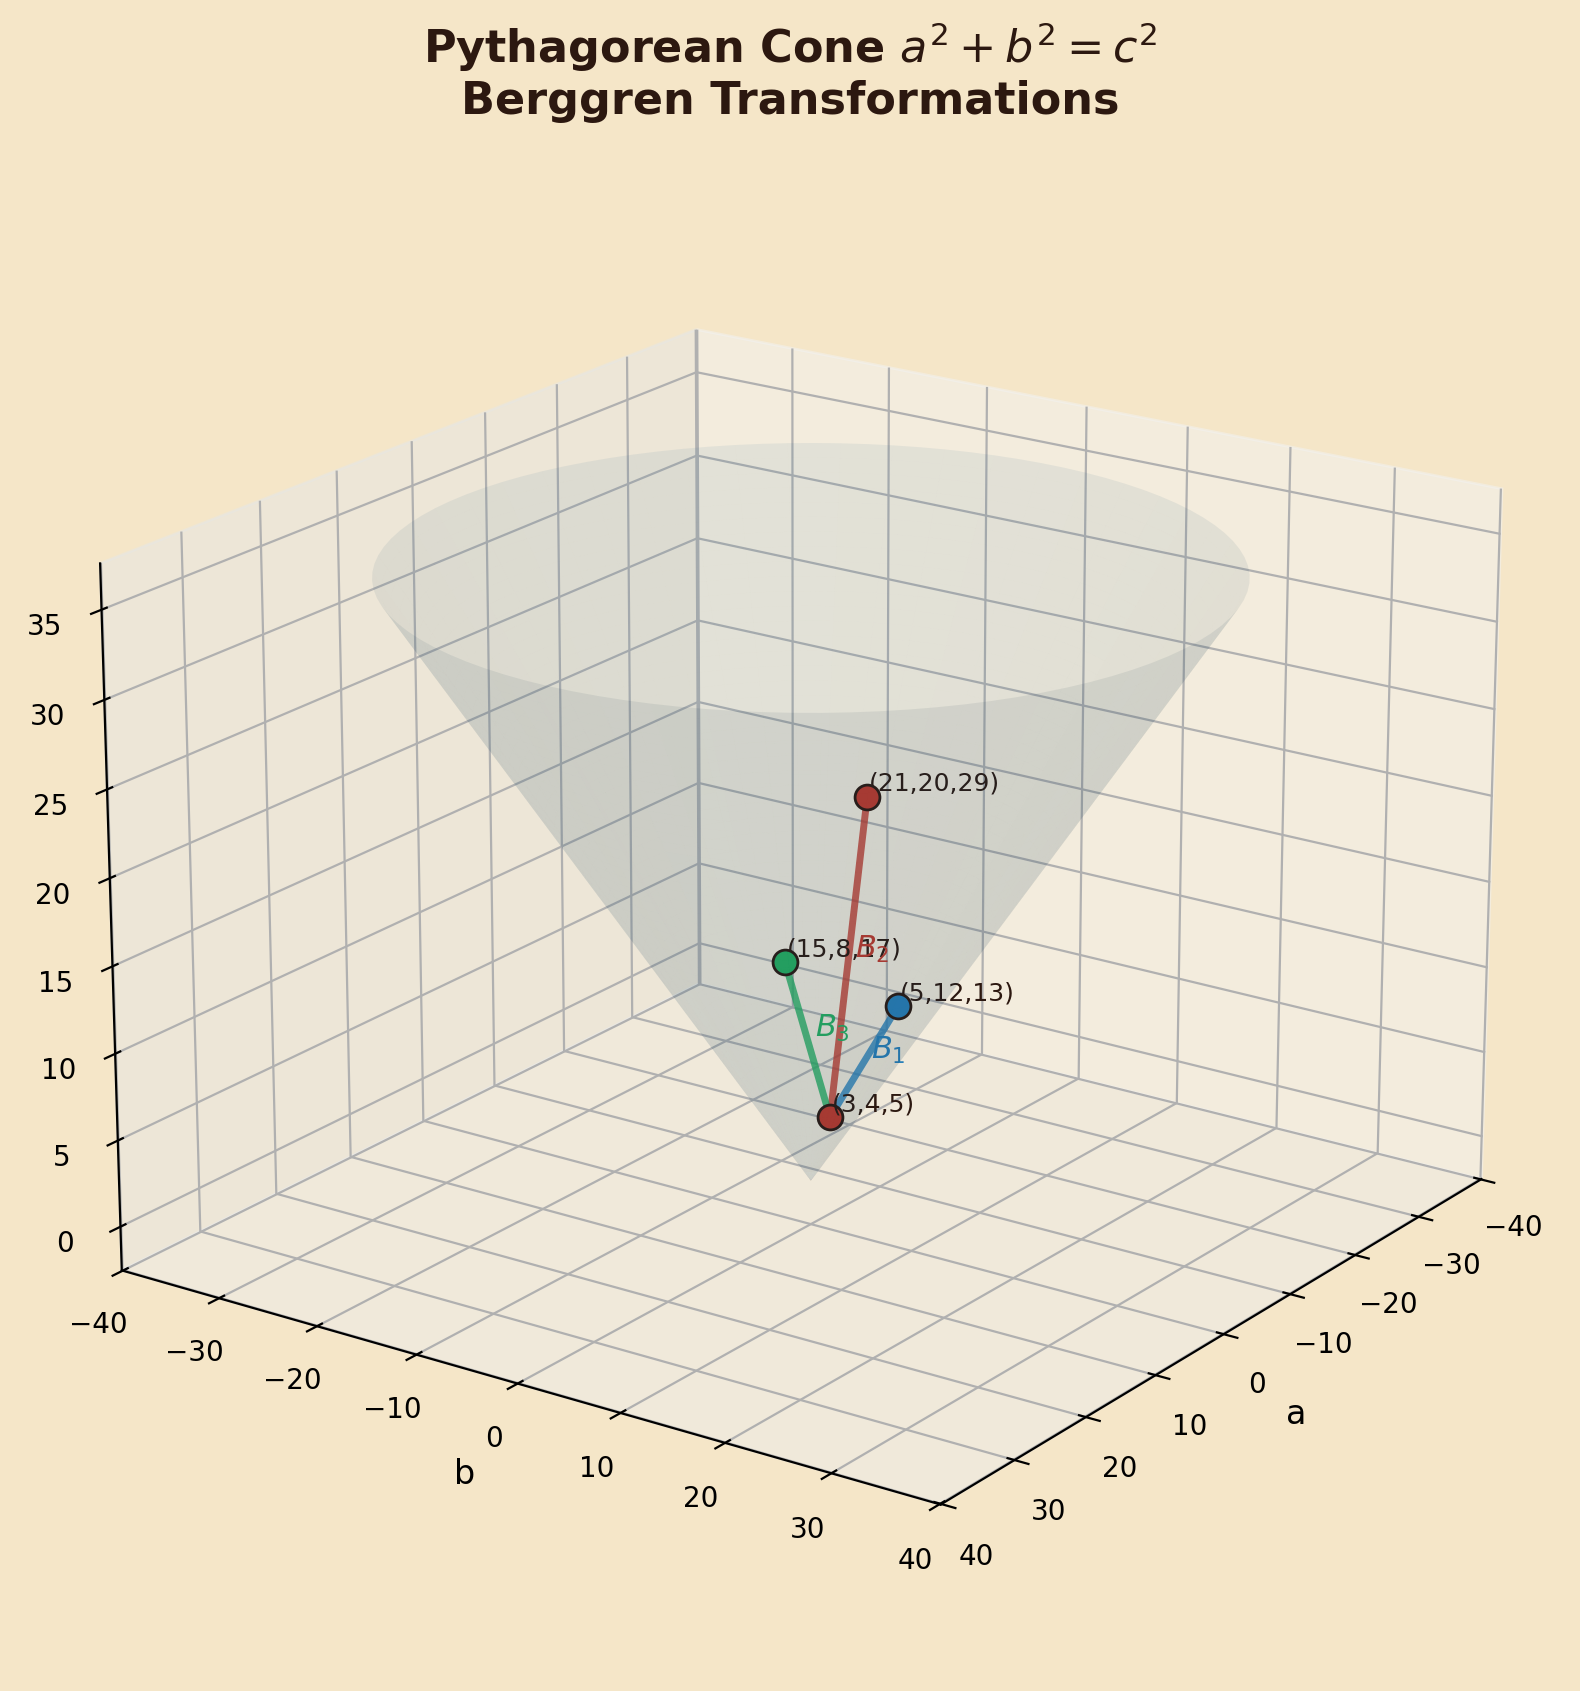
\includegraphics[width=0.85\textwidth]{Chapter4/images/fig07_pythagorean_cone.png}
\caption{}
\end{figure}
A three-dimensional perspective drawing of the cone \(x^2 + y^2 = z^2\) rising upward from the origin. The surface is translucent, revealing a grid of integer lattice points. The point \((3, 4, 5)\) is labeled at the root, and three arrows --- colored blue (\(B_1\)), red (\(B_2\)), and green (\(B_3\)) --- arc along the cone's surface to three new lattice points: \((5, 12, 13)\), \((21, 20, 29)\), and \((15, 8, 17)\). All four points sit precisely on the cone's surface. Faint grid lines on the cone show its ruled structure.{]}

This connection between Pythagoras and Einstein is not merely cosmetic. In special relativity, a Lorentz transformation is a change of reference frame --- moving from one observer's coordinate system to another's --- that preserves the \emph{spacetime interval} \(x^2 + y^2 - t^2\) (in natural units where \(c = 1\)). The surfaces where this interval vanishes are \emph{light cones}: the boundaries between events that can communicate by light signals and events that cannot. The Berggren matrices are doing the same thing in integer arithmetic: they are ``changes of reference frame'' that map the Pythagorean cone to itself, jumping from one lattice point to another.


\begin{figure}[htbp]
\centering
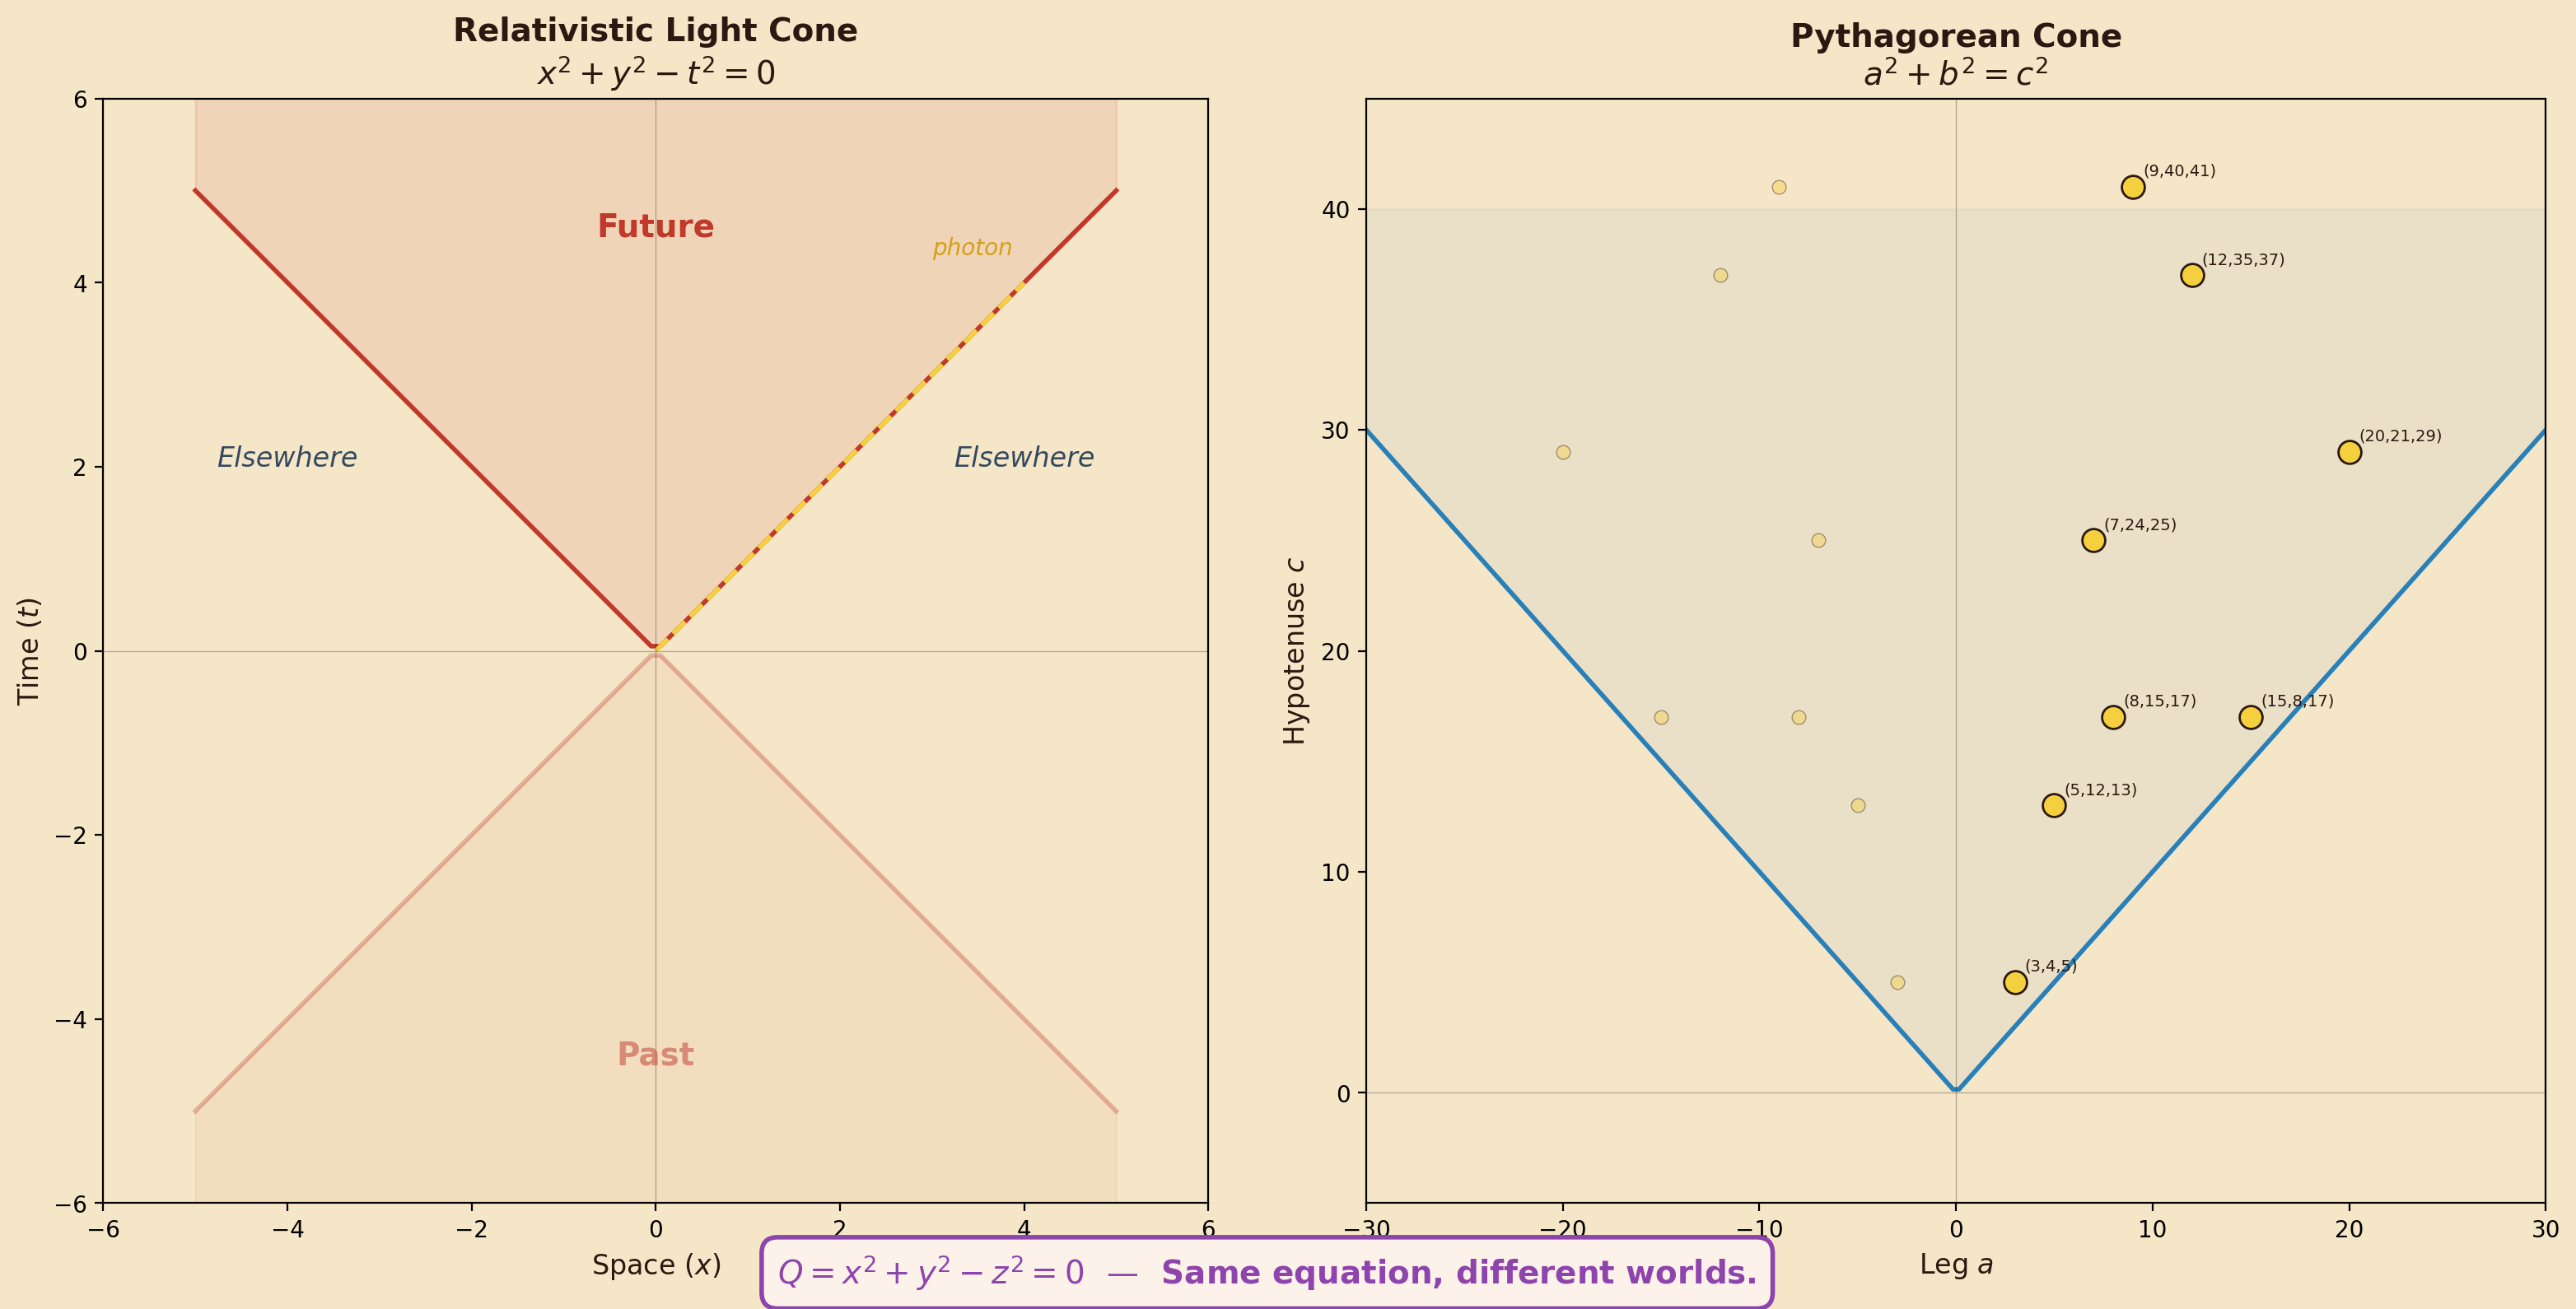
\includegraphics[width=0.85\textwidth]{Chapter4/images/fig08_light_cones.png}
\caption{}
\end{figure}
A side-by-side comparison. LEFT: A relativistic light cone in \(2+1\) spacetime dimensions, with a photon worldline traced along the cone's surface and labels for ``future,'' ``past,'' and ``elsewhere.'' RIGHT: The Pythagorean cone \(a^2 + b^2 = c^2\) with integer lattice points glowing on its surface, each labeled with a familiar triple. Between the two images, a bridge labeled ``\(Q = x^2 + y^2 - z^2 = 0\)'' connects them. The caption reads: ``Same equation, different worlds.''{]}

Physicists call this type of symmetry \emph{Lorentz invariance}, and it is one of the cornerstones of modern physics. The Berggren transformations are, in a precise sense, ``quantized'' Lorentz boosts --- discrete jumps rather than continuous rotations, but obeying the same fundamental constraint. The ancient theorem of Pythagoras and the modern theory of spacetime are branches of the same mathematical tree.

\bigskip\noindent\rule{\linewidth}{0.4pt}\bigskip

\section{The Berggren Tree --- An Infinite Family Album}
Start with \((3, 4, 5)\). Apply \(B_1\), \(B_2\), and \(B_3\). You now have three children:

\[B_1(3, 4, 5) = (5, 12, 13), \quad B_2(3, 4, 5) = (21, 20, 29), \quad B_3(3, 4, 5) = (15, 8, 17).\]

Apply all three transformations to each child, and you get nine grandchildren. Apply again, and you get twenty-seven great-grandchildren. The tree branches without end.

Here are the first three levels, computed explicitly:

\begin{longtable}[]{@{}cll@{}}
\toprule\noalign{}
Level & Triple & Parent \\
\midrule\noalign{}
\endhead
\bottomrule\noalign{}
\endlastfoot
0 & \((3, 4, 5)\) & --- \\
1 & \((5, 12, 13)\) & \(B_1(3,4,5)\) \\
1 & \((21, 20, 29)\) & \(B_2(3,4,5)\) \\
1 & \((15, 8, 17)\) & \(B_3(3,4,5)\) \\
2 & \((7, 24, 25)\) & \(B_1(5,12,13)\) \\
2 & \((55, 48, 73)\) & \(B_2(5,12,13)\) \\
2 & \((45, 28, 53)\) & \(B_3(5,12,13)\) \\
2 & \((39, 80, 89)\) & \(B_1(21,20,29)\) \\
2 & \((119, 120, 169)\) & \(B_2(21,20,29)\) \\
2 & \((77, 36, 85)\) & \(B_3(21,20,29)\) \\
2 & \((9, 40, 41)\) & \(B_1(15,8,17)\) \\
2 & \((65, 72, 97)\) & \(B_2(15,8,17)\) \\
2 & \((35, 12, 37)\) & \(B_3(15,8,17)\) \\
\end{longtable}

Every primitive Pythagorean triple appears in this tree exactly once. No omissions, no repetitions. The tree is a perfect enumeration --- an infinite family album in which every member of the family has a unique portrait and a unique address (a finite sequence of branch labels \(B_1, B_2, B_3\) tracing the path from the root).


\begin{figure}[htbp]
\centering
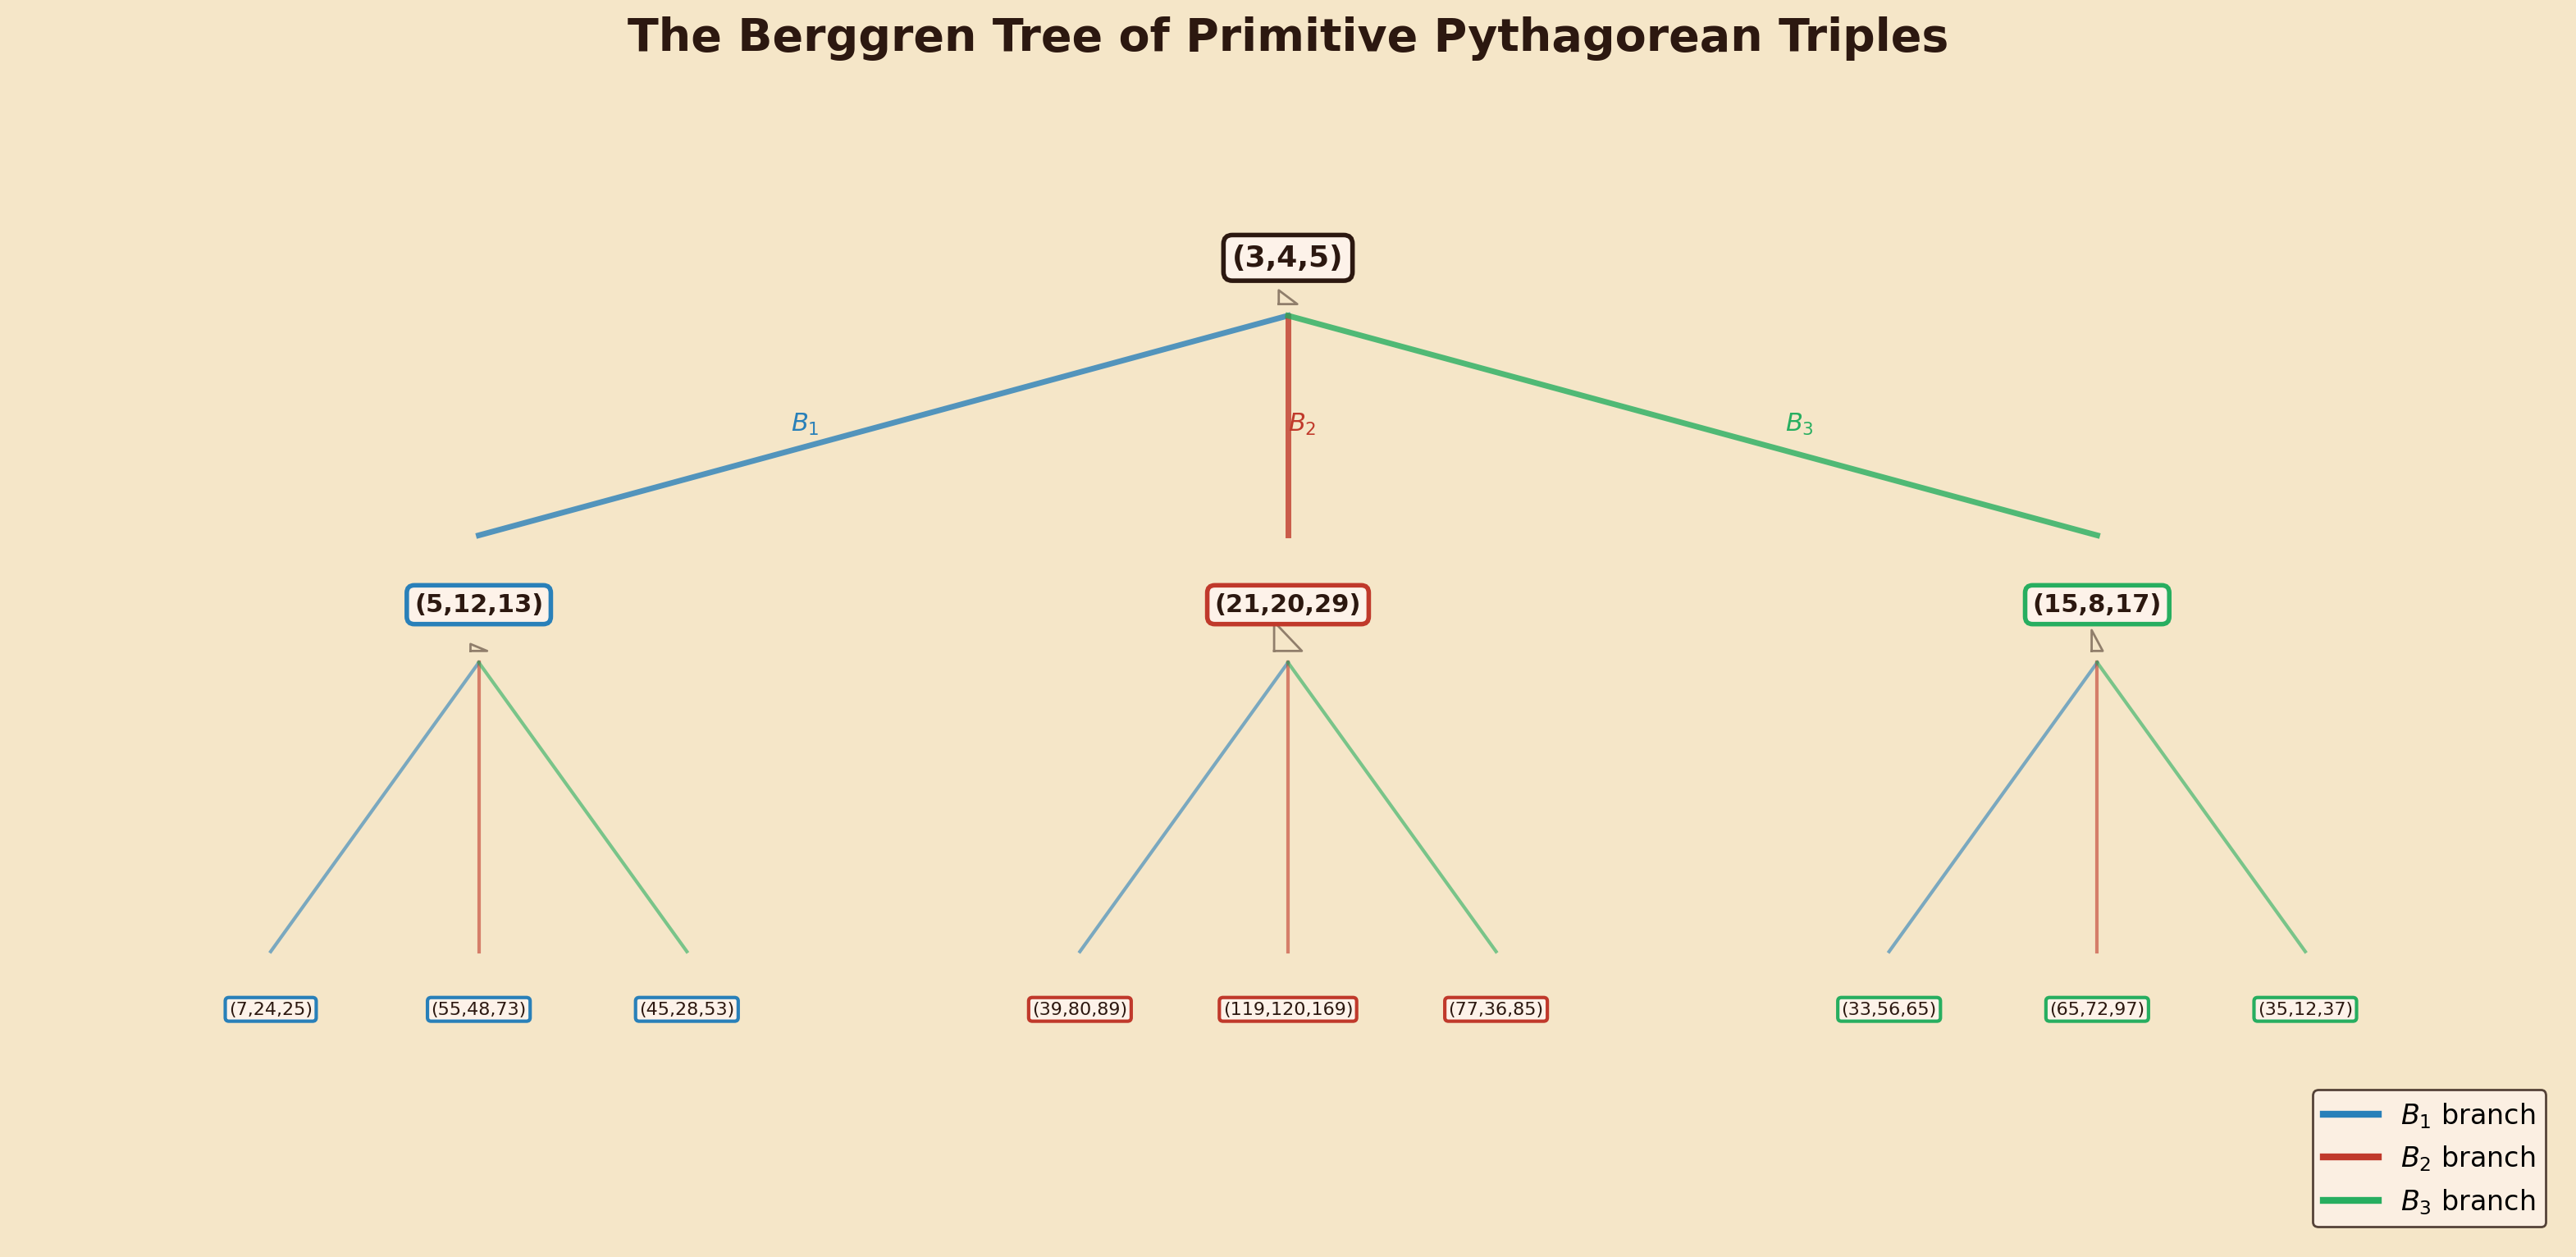
\includegraphics[width=0.85\textwidth]{Chapter4/images/fig09_berggren_tree.png}
\caption{}
\end{figure}
A full ternary tree, three levels deep. The root node at the top contains \((3, 4, 5)\) with a small right triangle drawn to scale. Three branches descend, colored blue (\(B_1\)), red (\(B_2\)), and green (\(B_3\)). Each of the three Level-1 nodes contains its triple and a scaled right triangle. Nine Level-2 nodes fan out below, again color-coded by their parent branch. The overall shape evokes a family genealogy chart, with the triangles growing in size as the hypotenuses increase.{]}

The history of this tree is a case study in mathematical rediscovery. B. Berggren, a Swedish schoolteacher, published the result in 1934 in a Swedish-language journal of such limited circulation that the mathematical world scarcely noticed. His paper proved that the three transformations generate every primitive triple from the seed \((3, 4, 5)\) --- a complete, constructive enumeration of an infinite set hidden in the most classical corner of number theory. Decades passed. In 1963, F. J. M. Barning rediscovered the tree independently. In 1970, A. Hall did it again. Today the Berggren tree is a staple of recreational mathematics and computational number theory, but its original discoverer, as far as anyone knows, never learned how famous his tree would become.

Why does the tree cover everything? The essential argument runs in reverse. Given any primitive Pythagorean triple other than \((3, 4, 5)\), exactly one of the three \emph{inverse} transformations \(B_1^{-1}\), \(B_2^{-1}\), \(B_3^{-1}\) produces a new primitive triple with a \emph{smaller} hypotenuse. Repeat. Since the hypotenuse strictly decreases at each step and is bounded below by \(5\), the process must eventually reach \((3, 4, 5)\). The path you traced defines the triple's unique address in the tree.

\bigskip\noindent\rule{\linewidth}{0.4pt}\bigskip

\section{The Tree Sieve --- Shaking the Family Tree for Factors}
Here is a puzzle. Given \(N = 31{,}861\), factor it.

You could try trial division --- testing every prime up to \(\sqrt{31861} \approx 178\). That works, but it is tedious. I want to show you a method that uses the Berggren tree as a sieve.

The key observation is this. If we can find integers \(b\) and \(c\) such that

\[N^2 + b^2 = c^2,\]

then \((c - b)(c + b) = N^2\). The values \(d_1 = c - b\) and \(d_2 = c + b\) are a complementary pair of divisors of \(N^2\), and if we are lucky, \(\gcd(d_1, N)\) or \(\gcd(d_2, N)\) will be a non-trivial factor of \(N\) --- not \(1\) and not \(N\) itself.

\textbf{Tree Sieve Divisor Theorem.} If \(N^2 + b^2 = c^2\), then \((c - b)(c + b) = N^2\). If \(d = c - b\) satisfies \(1 < \gcd(d, N) < N\), then \(\gcd(d, N)\) is a non-trivial factor of \(N\).

The Berggren tree enters the picture because every Pythagorean triple \((a, b, c)\) satisfies \((c - b)(c + b) = a^2\), and we can walk the tree looking for triples where \(a\) shares a factor with our target \(N\). When we find such a triple, we compute \(\gcd(a, N)\) and hope it splits \(N\).


\begin{figure}[htbp]
\centering
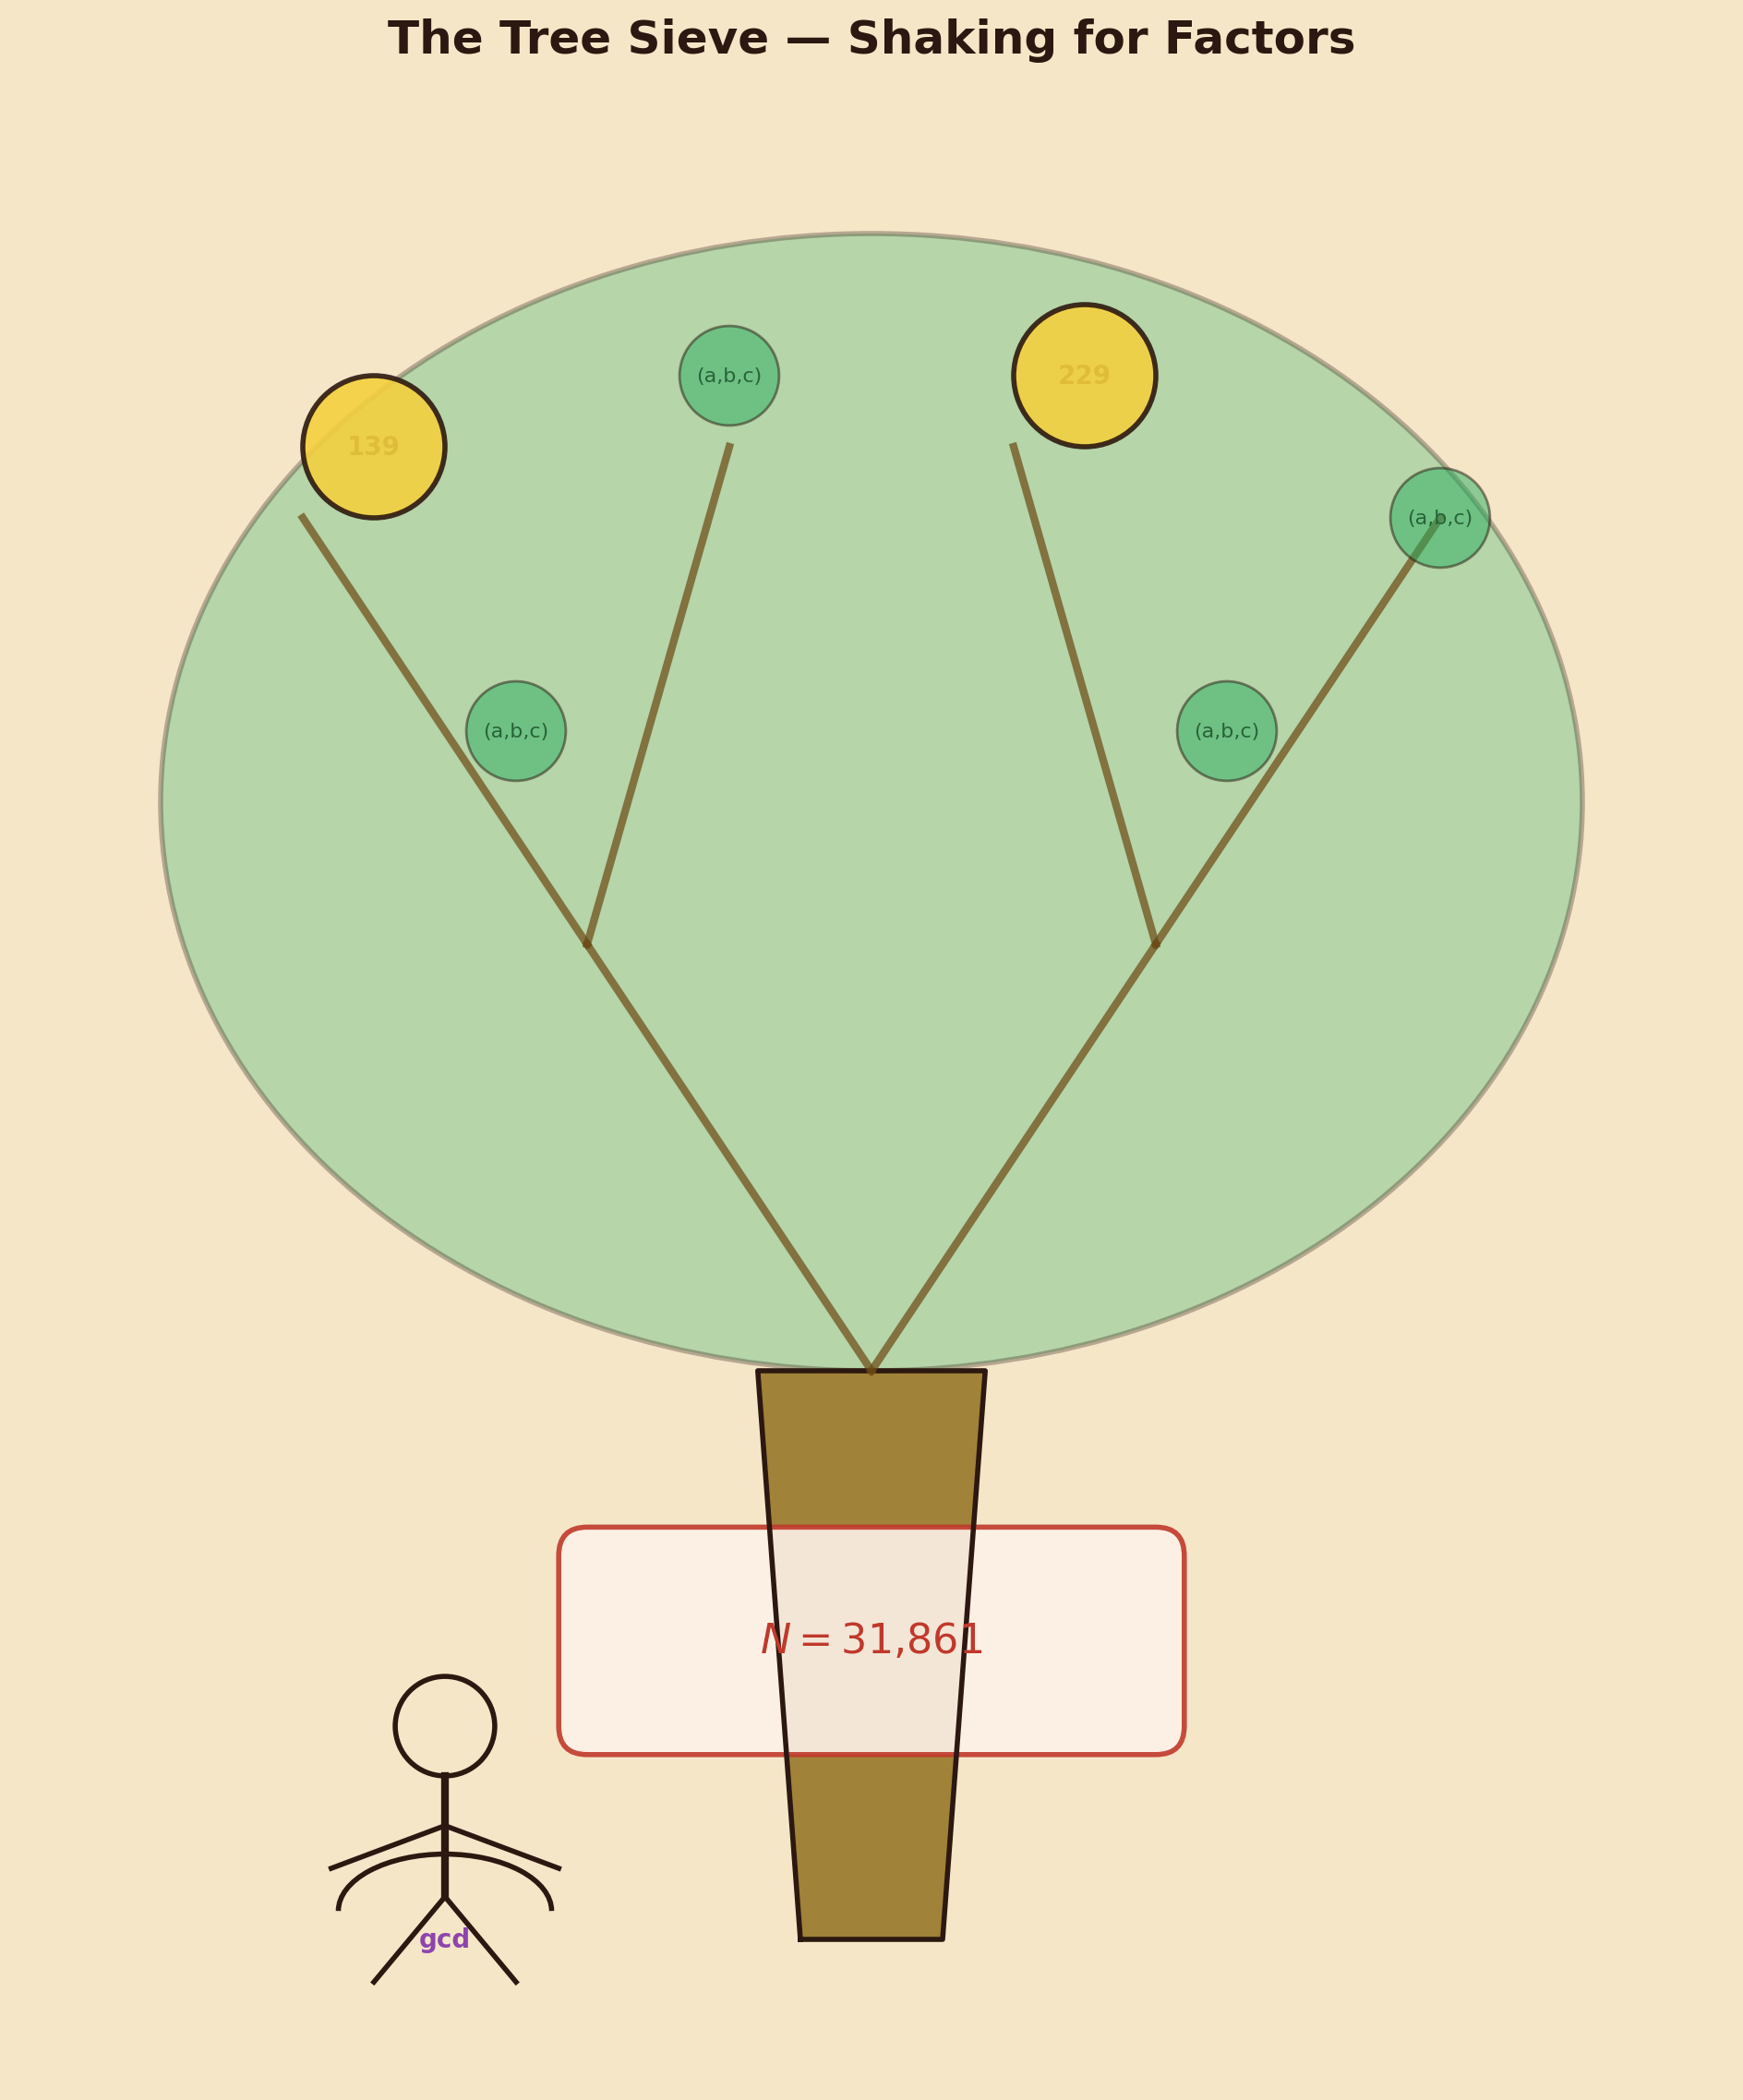
\includegraphics[width=0.85\textwidth]{Chapter4/images/fig10_tree_sieve.png}
\caption{}
\end{figure}
A stylized tree with thick trunk and spreading branches. Some branches bear glowing ``fruit'' --- small spheres labeled with divisor values. At the base of the tree, a figure in a mathematician's robe holds a basket labeled ``\(\gcd\).'' The highlighted branches carry Pythagorean triples whose leg \(a\) shares a factor with a target number \(N\) displayed on a banner draped across the trunk.{]}

For our example, \(N = 31{,}861\): a search through the early levels of the Berggren tree turns up triples whose legs share factors with \(N\). Computing GCDs reveals \(31{,}861 = 139 \times 229\). The tree has shaken loose the factors.


\begin{figure}[htbp]
\centering
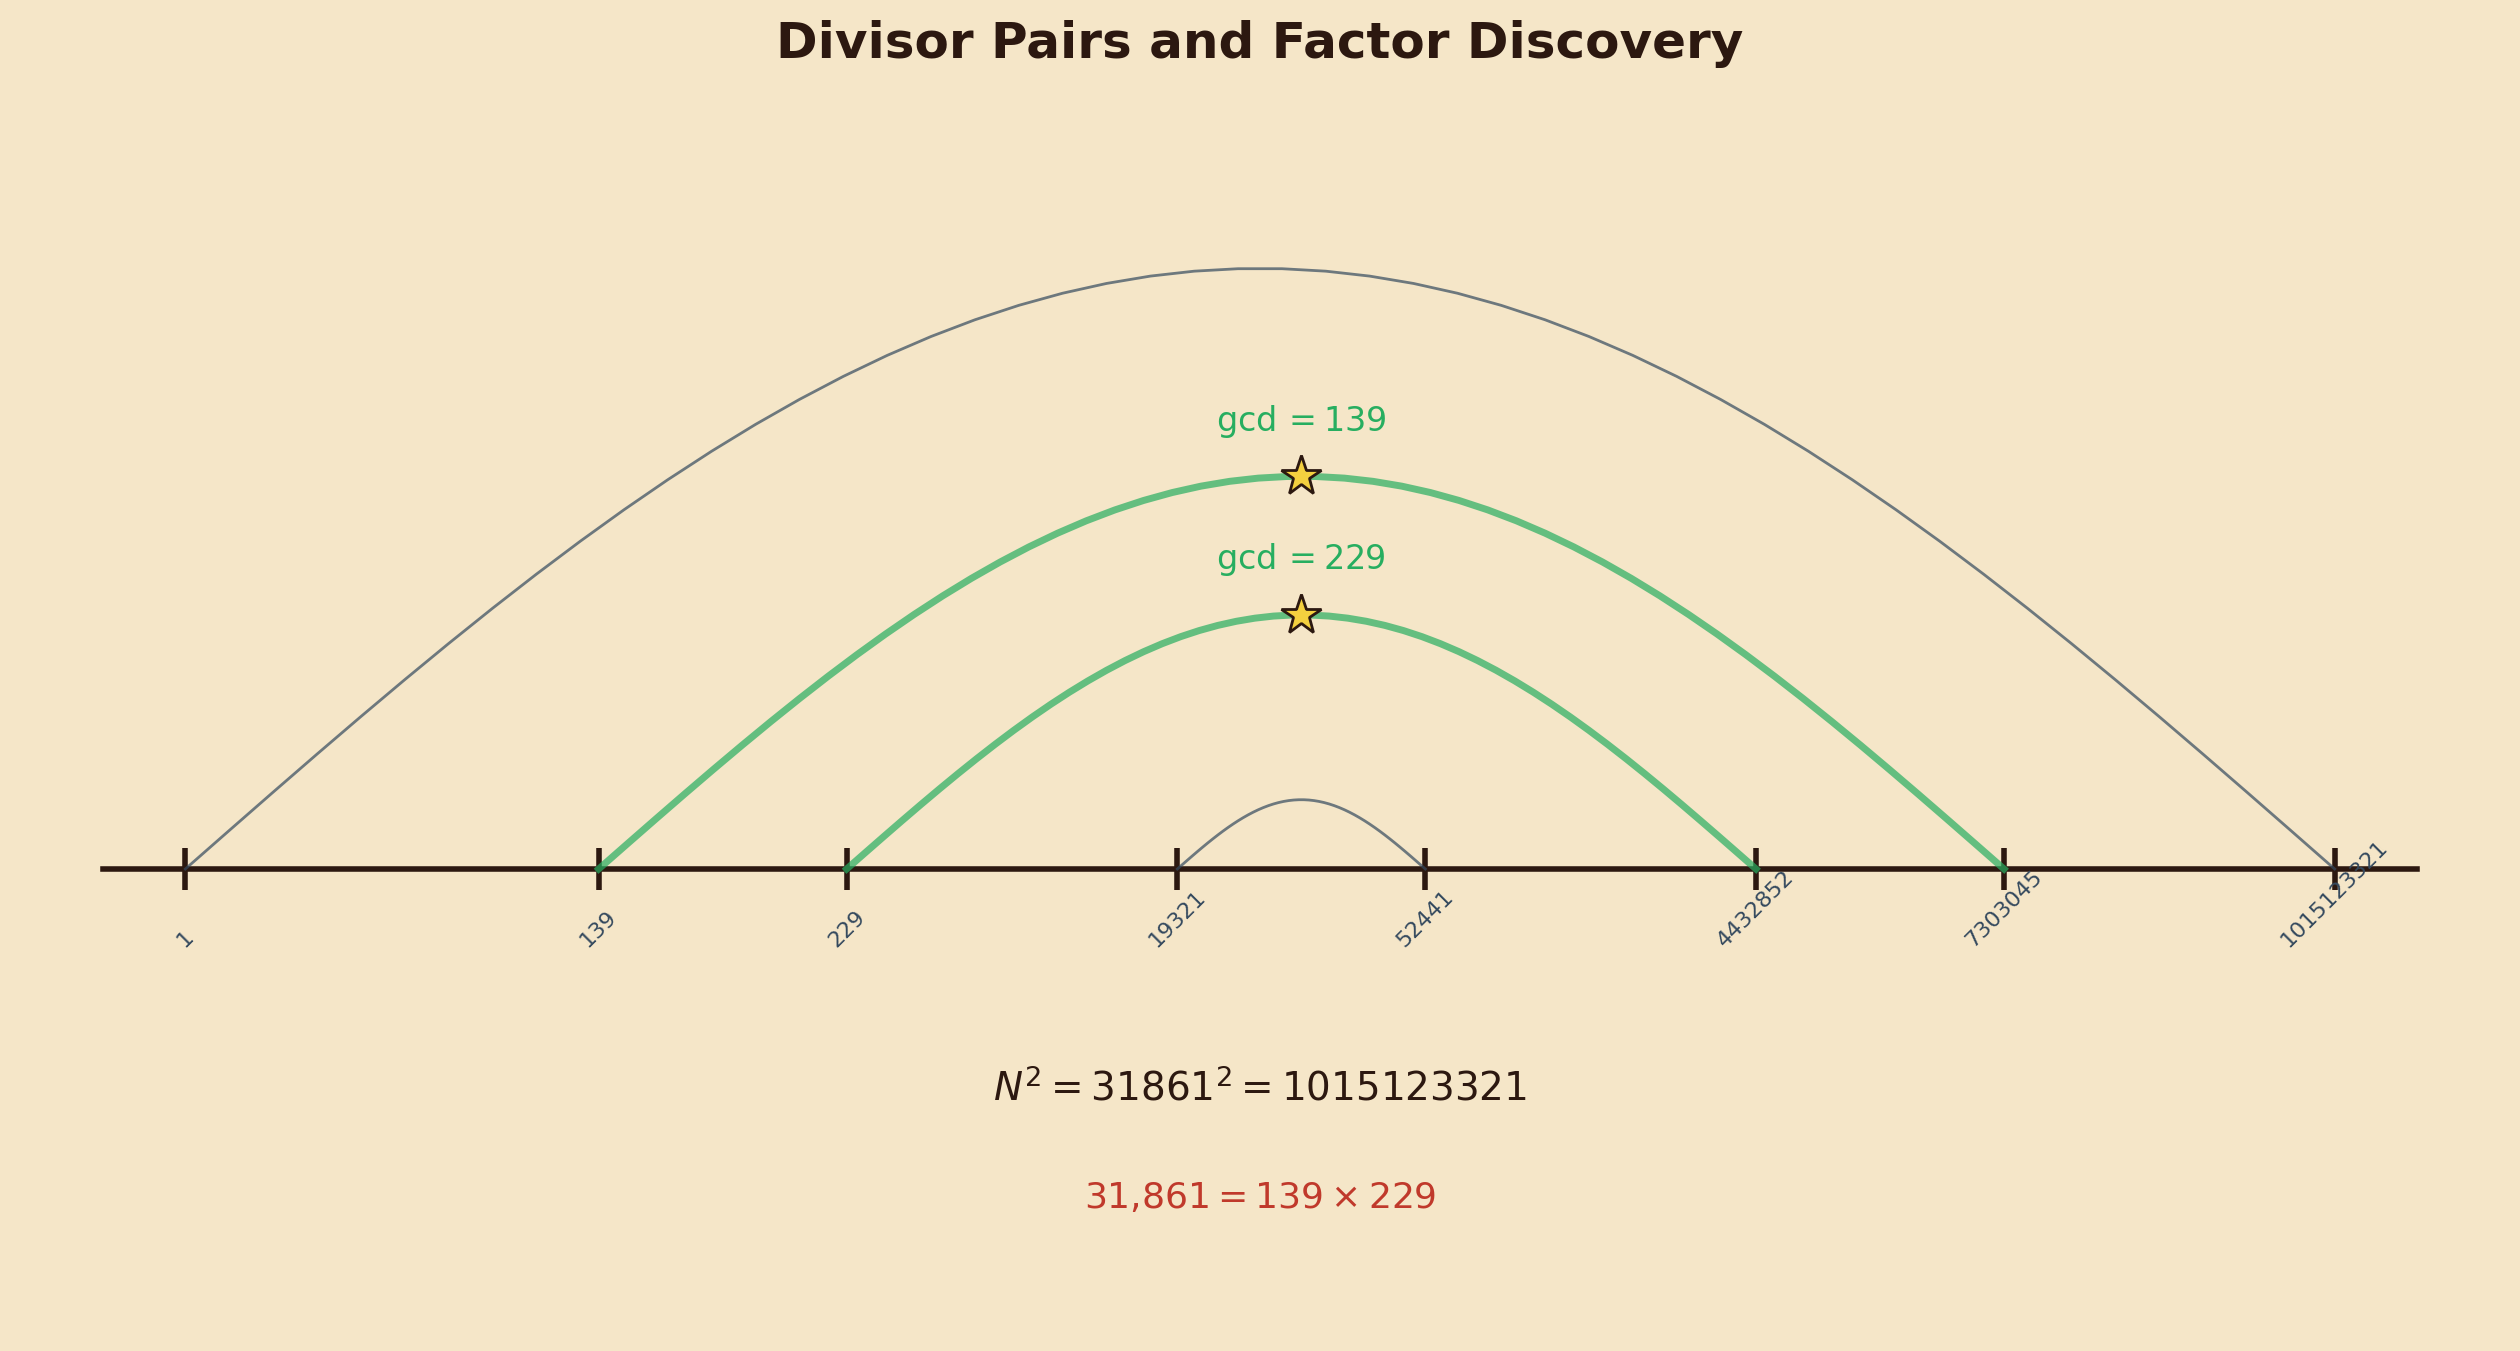
\includegraphics[width=0.85\textwidth]{Chapter4/images/fig11_divisor_arcs.png}
\caption{}
\end{figure}
A number line showing \(N^2 = 31861^2\) with tick marks at selected divisor pairs. Arcs connect complementary pairs \((c - b, c + b)\) that multiply to \(N^2\). Stars mark the positions where arcs reveal non-trivial factors of \(N\). Two particular arcs are highlighted, one yielding \(\gcd = 139\) and the other yielding \(\gcd = 229\).{]}

The strategy generalizes. Walk the tree level by level. At each node, check whether the triple's legs share a factor with \(N\). If so, you've found your splitting. If not, keep climbing. The Brahmagupta--Fibonacci composition can accelerate the search: combine triples whose residues modulo \(N\) are ``smooth'' (divisible only by small primes), and the composition may produce a triple that directly reveals a factor.

\bigskip\noindent\rule{\linewidth}{0.4pt}\bigskip

\section{\texorpdfstring{Semiprime Secrets --- Why \(N = p \times q\) Is Special}{Semiprime Secrets --- Why N = p \textbackslash times q Is Special}}
The entire edifice of internet security rests on one assumption: given a large number \(N = pq\), the product of two large primes, recovering \(p\) and \(q\) is computationally infeasible.

Every time you type a credit card number into a website, every time your browser displays the little padlock icon, a semiprime is standing guard. The RSA cryptosystem --- named after Rivest, Shamir, and Adleman, who published it in 1978 --- relies on the practical impossibility of factoring a number that is the product of two primes, each several hundred digits long.

Why are semiprimes special for our purposes? Because when \(N = pq\), the number \(N^2 = p^2 q^2\) has at least two genuinely different factorizations: \(1 \cdot N^2\) and \(p^2 \cdot q^2\). These are distinct whenever \(p > 1\) (which it always is, since \(p\) is prime). And each factorization of \(N^2\) into a product \(d_1 \cdot d_2\) corresponds, via \(d_1 = c - b\) and \(d_2 = c + b\), to a Pythagorean triple with leg \(N\). Two different factorizations, two different triples, two different sum-of-squares representations --- and we have seen what Euler does with two representations.

This is the conceptual bridge that connects ancient geometry to modern cryptography. The three roads from Pythagoras converge:

\textbf{Road 1 --- Euler's Two Portraits.} If you can express \(N\) (or \(N^2\)) as a sum of two squares in two different ways, Euler's method extracts a non-trivial factor.

\textbf{Road 2 --- Gaussian Composition.} The Brahmagupta--Fibonacci identity lets you \emph{manufacture} new sum-of-squares representations by composing existing ones, amplifying partial information into a full factorization.

\textbf{Road 3 --- The Berggren Tree Sieve.} Systematically walk the tree of Pythagorean triples, collecting those whose legs relate to \(N\), and combine them to extract factors.


\begin{figure}[htbp]
\centering
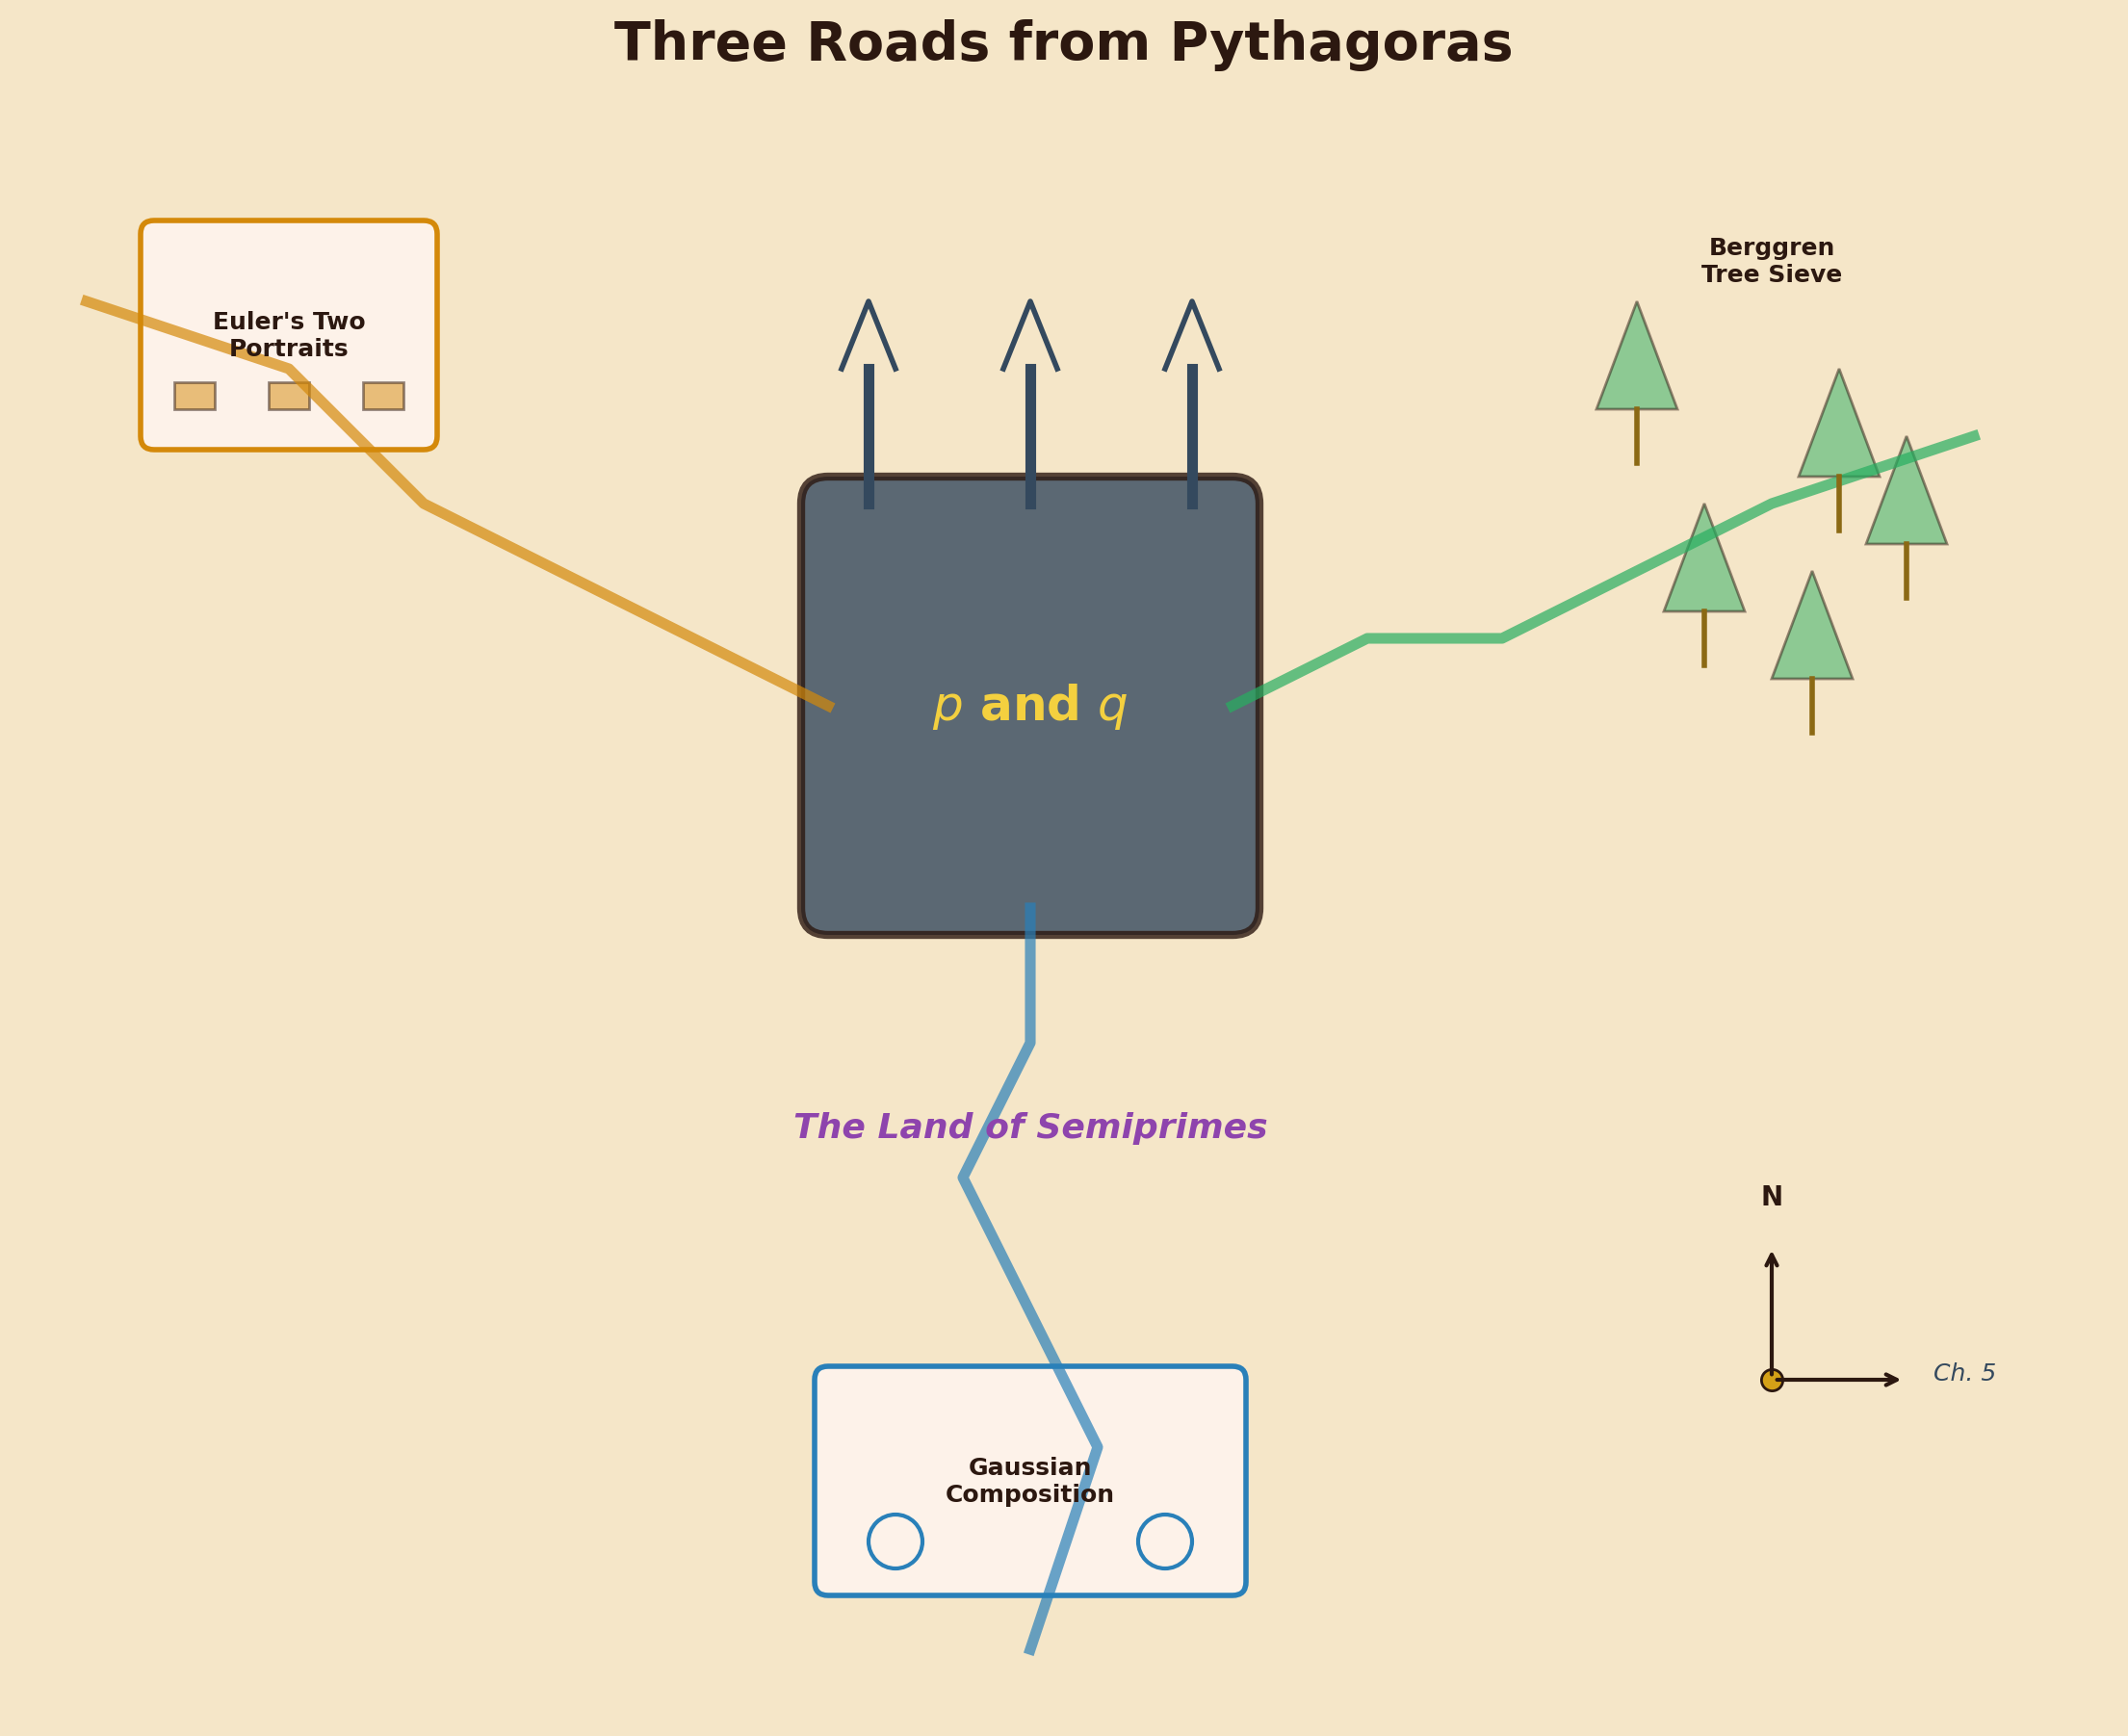
\includegraphics[width=0.85\textwidth]{Chapter4/images/fig12_three_roads_map.png}
\caption{}
\end{figure}
A stylized map drawn in the manner of a medieval cartographer. Three winding roads converge on a fortified castle at the center, labeled ``\(p\) and \(q\).'' Road 1, ``Euler's Two Portraits,'' passes through an art gallery with portraits on the walls showing different sum-of-squares representations. Road 2, ``Gaussian Composition,'' winds through a factory floor where triangles are being combined on assembly lines. Road 3, ``The Berggren Tree Sieve,'' threads through a dense forest of branching trees. The landscape around the castle is labeled ``The Land of Semiprimes.'' A compass rose in the corner points toward ``Chapter 5'' to the east.{]}

\bigskip\noindent\rule{\linewidth}{0.4pt}\bigskip

\section{The Exponential Climb --- How Fast the Tree Grows}
Each generation of the Berggren tree at least \emph{triples} the hypotenuse. By the twentieth generation, you've passed a billion.

To see why, look at the formula for \(c'\) in any of the three transformations. Taking \(B_2\) as representative:

\[c' = 2a + 2b + 3c.\]

Since \(a \geq 0\) and \(b \geq 0\) for any triple in the tree, we have \(c' \geq 3c\). This is the \textbf{Hypotenuse Growth Lemma}: every step at least triples the hypotenuse.

Iterating, after \(k\) steps: \(c_k \geq 3^k \cdot c_0 = 3^k \cdot 5\).

\begin{longtable}[]{@{}
  >{\centering\arraybackslash}p{(\columnwidth - 4\tabcolsep) * \real{0.3333}}
  >{\raggedright\arraybackslash}p{(\columnwidth - 4\tabcolsep) * \real{0.3333}}
  >{\raggedright\arraybackslash}p{(\columnwidth - 4\tabcolsep) * \real{0.3333}}@{}}
\toprule\noalign{}
\begin{minipage}[b]{\linewidth}\centering
Generation \(k\)
\end{minipage} & \begin{minipage}[b]{\linewidth}\raggedright
Lower bound \(3^k \cdot 5\)
\end{minipage} & \begin{minipage}[b]{\linewidth}\raggedright
Actual maximum \(c\) in generation
\end{minipage} \\
\midrule\noalign{}
\endhead
\bottomrule\noalign{}
\endlastfoot
0 & 5 & 5 \\
1 & 15 & 29 \\
2 & 45 & 169 \\
3 & 135 & 985 \\
5 & 1,215 & \(\sim 33{,}000\) \\
10 & \(\sim 295{,}000\) & \(\sim 10^7\) \\
20 & \(\sim 1.7 \times 10^{10}\) & \(\sim 10^{14}\) \\
40 & \(\sim 6 \times 10^{19}\) & \(\sim 10^{29}\) \\
\end{longtable}

The tree grows exponentially, reaching any target \(N\) in roughly \(\log_3 N\) generations. But --- and this is the crucial ``but'' --- the number of \emph{nodes} at generation \(k\) is \(3^k\), and finding the \emph{right} node among them requires searching an exponentially large haystack. The tree reaches \(N\) quickly in depth, but finding the needle requires \(\sim \sqrt{N}\) work. This is no better than trial division --- and no worse than the best known classical factoring algorithms for generic numbers.


\begin{figure}[htbp]
\centering
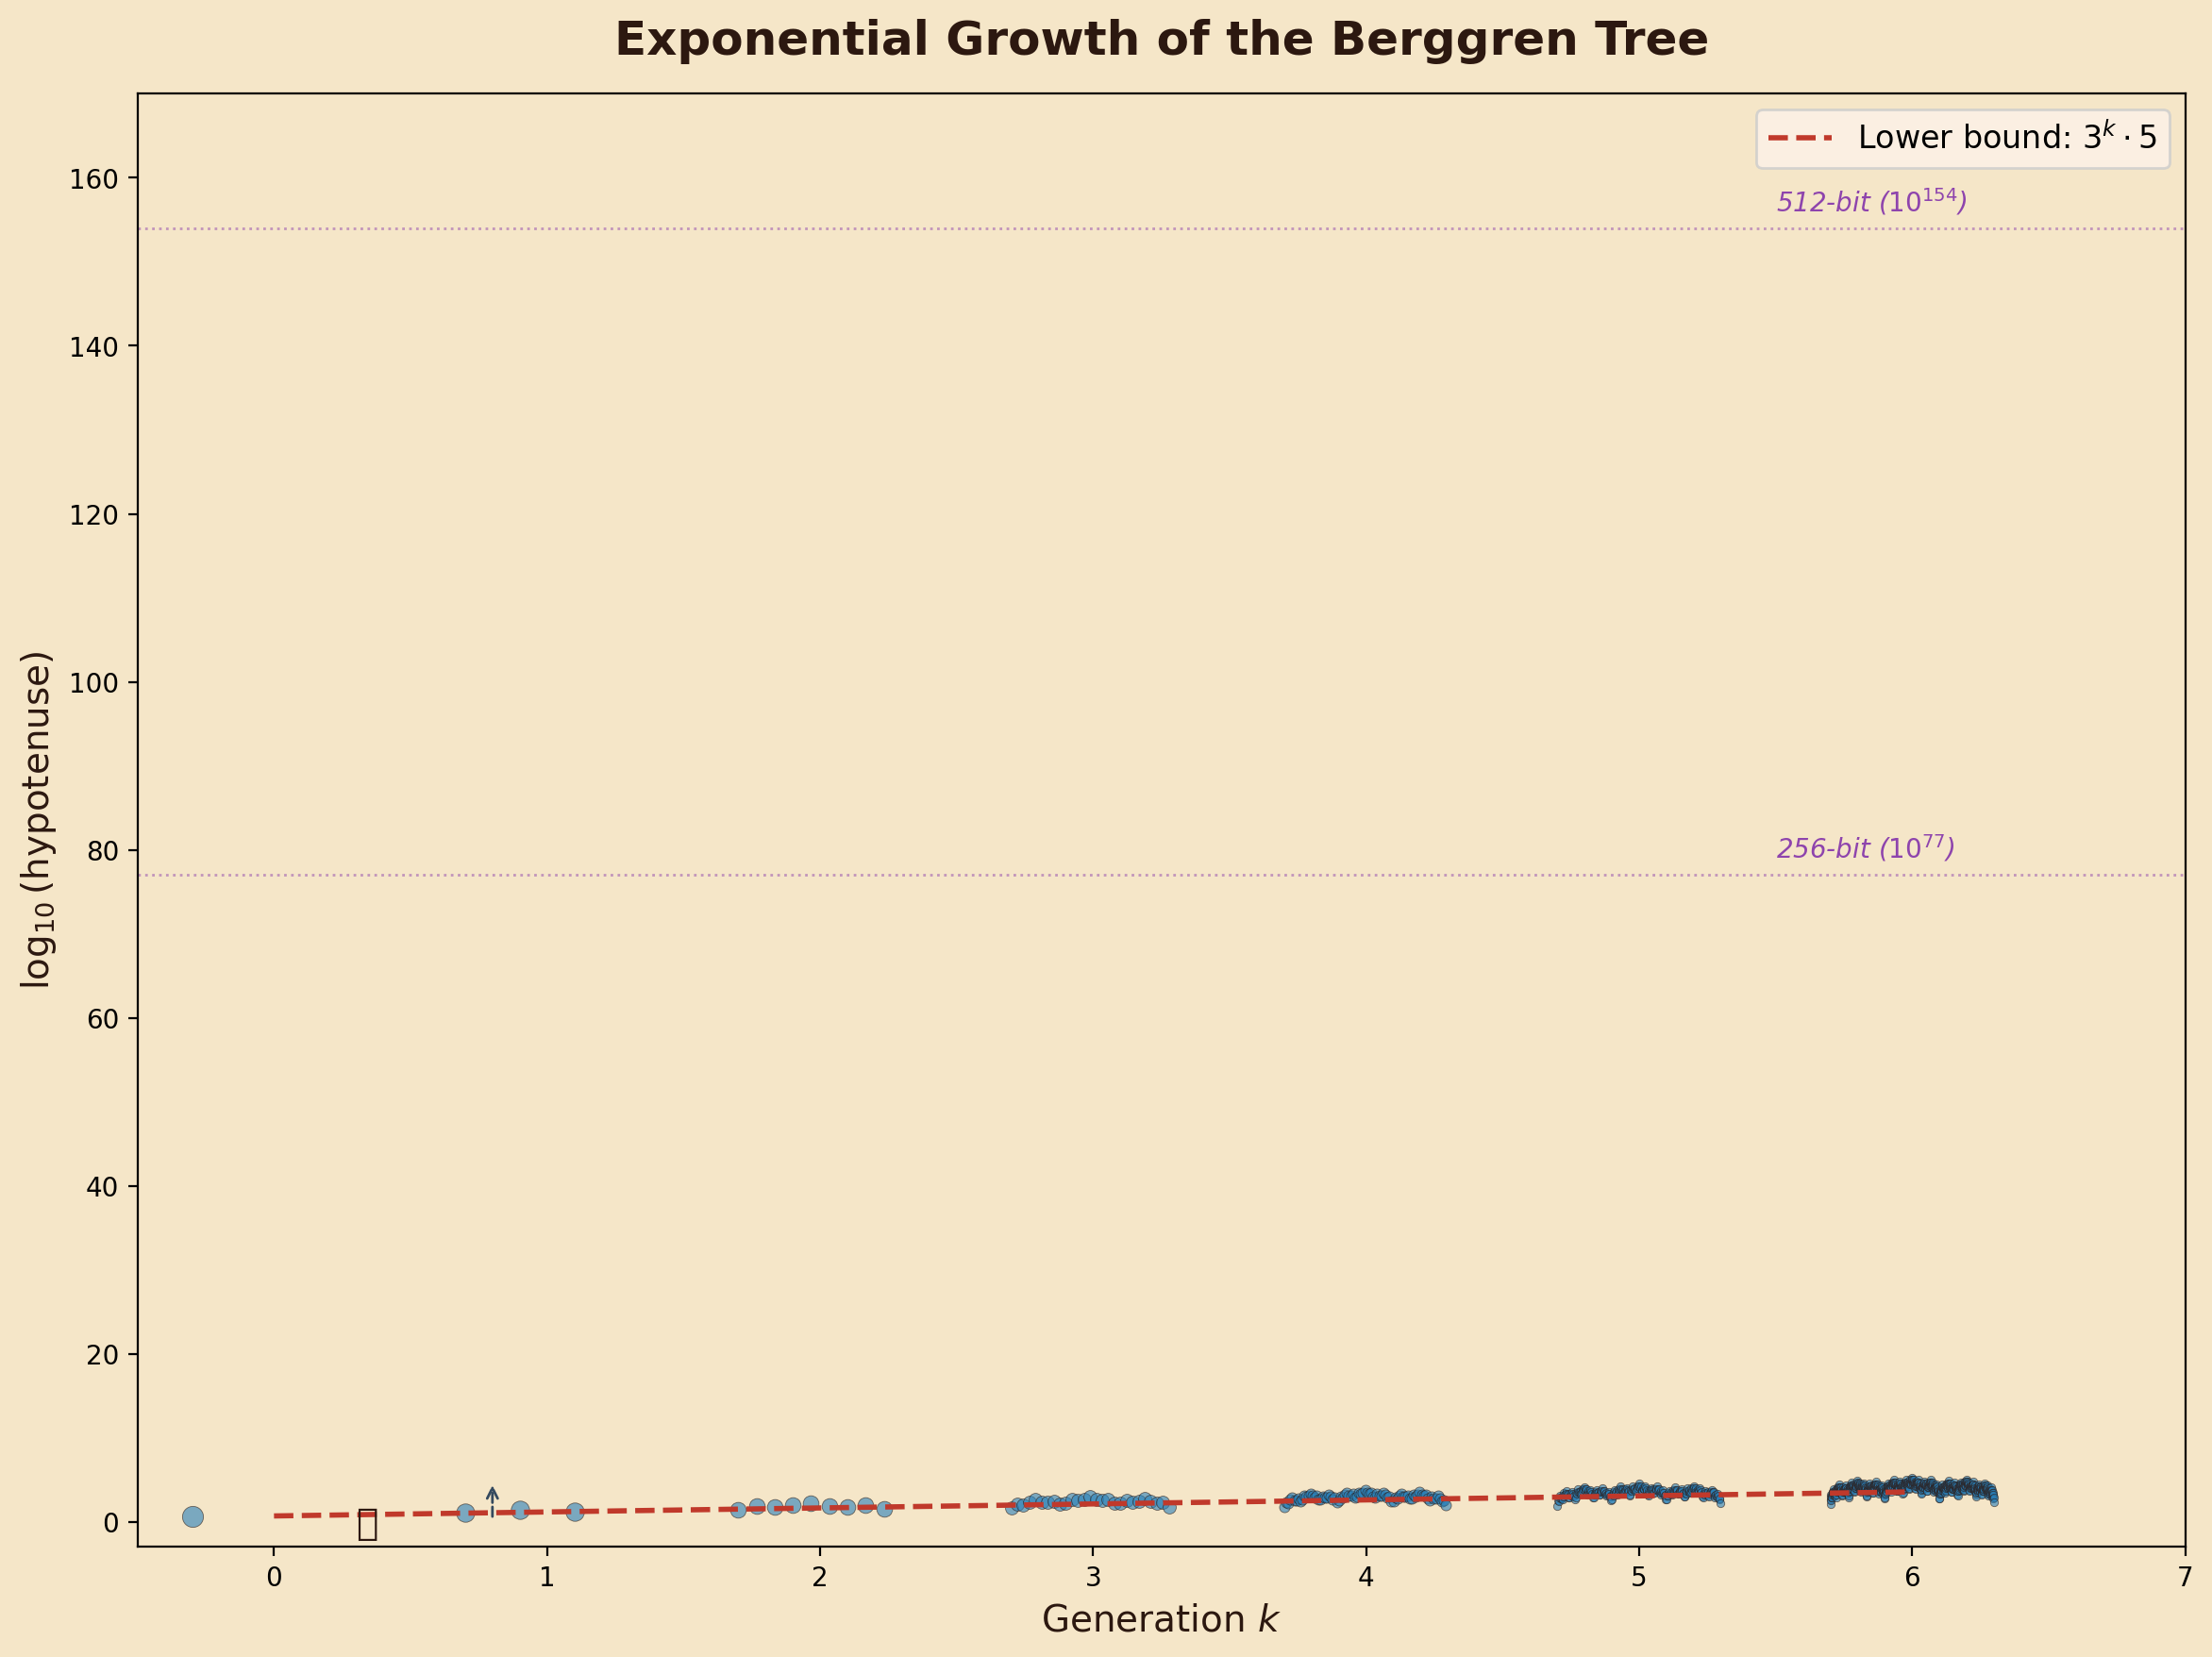
\includegraphics[width=0.85\textwidth]{Chapter4/images/fig13_exponential_climb.png}
\caption{}
\end{figure}
A vertical logarithmic scale running from \(10^0\) at the bottom to \(10^{20}\) at the top. The Berggren tree is drawn sideways, with the root at the left and branches extending to the right. The vertical position of each node corresponds to the logarithm of its hypotenuse. The tree fans out and rises steeply. Dashed horizontal lines mark RSA-size numbers: \(10^{77}\) (256-bit), \(10^{154}\) (512-bit), and \(10^{308}\) (1024-bit), all far above the visible portion of the tree. A small figure at the bottom looks up, shielding their eyes.{]}

\bigskip\noindent\rule{\linewidth}{0.4pt}\bigskip

\section{The Hidden Arithmetic of Products}
The products \(ab\) of Pythagorean triple legs, reduced modulo \(N\), form the smooth relations that power the tree sieve. But there is a beautiful bound constraining them.

\textbf{Product Bound (AM-GM).} For any Pythagorean triple \((a, b, c)\):

\[2ab \leq a^2 + b^2 = c^2.\]

The proof is a one-liner: \((a - b)^2 \geq 0\) implies \(a^2 + b^2 \geq 2ab\). Since \(a^2 + b^2 = c^2\), we have \(2ab \leq c^2\), or equivalently \(ab \leq c^2/2\). The product of the legs is always at most half the square of the hypotenuse.

This bound is tight when \(a = b\), i.e., for isosceles right triangles --- but those have \(c = a\sqrt{2}\), which is irrational, so no Pythagorean triple achieves exact equality. The near-isosceles triples \((20, 21, 29)\), \((119, 120, 169)\), \((697, 696, 985)\) --- the ones we met marching down the \(B_2\)-branch in Chapter 1 --- come closest, with \(ab/c^2\) approaching \(1/2\) from below.

Now comes the payoff. If \(N\) can be written as a sum of two squares in two different ways --- say \(N = a^2 + b^2 = c^2 + d^2\) --- then the Brahmagupta--Fibonacci identity gives us \emph{four} representations of \(N^2\):

\[N^2 = (ac + bd)^2 + (ad - bc)^2\] \[N^2 = (ac - bd)^2 + (ad + bc)^2\]

plus the two obtained by switching the roles of the pairs. Each representation is a potential key to unlock \(N\)'s factors via Euler's method.


\begin{figure}[htbp]
\centering
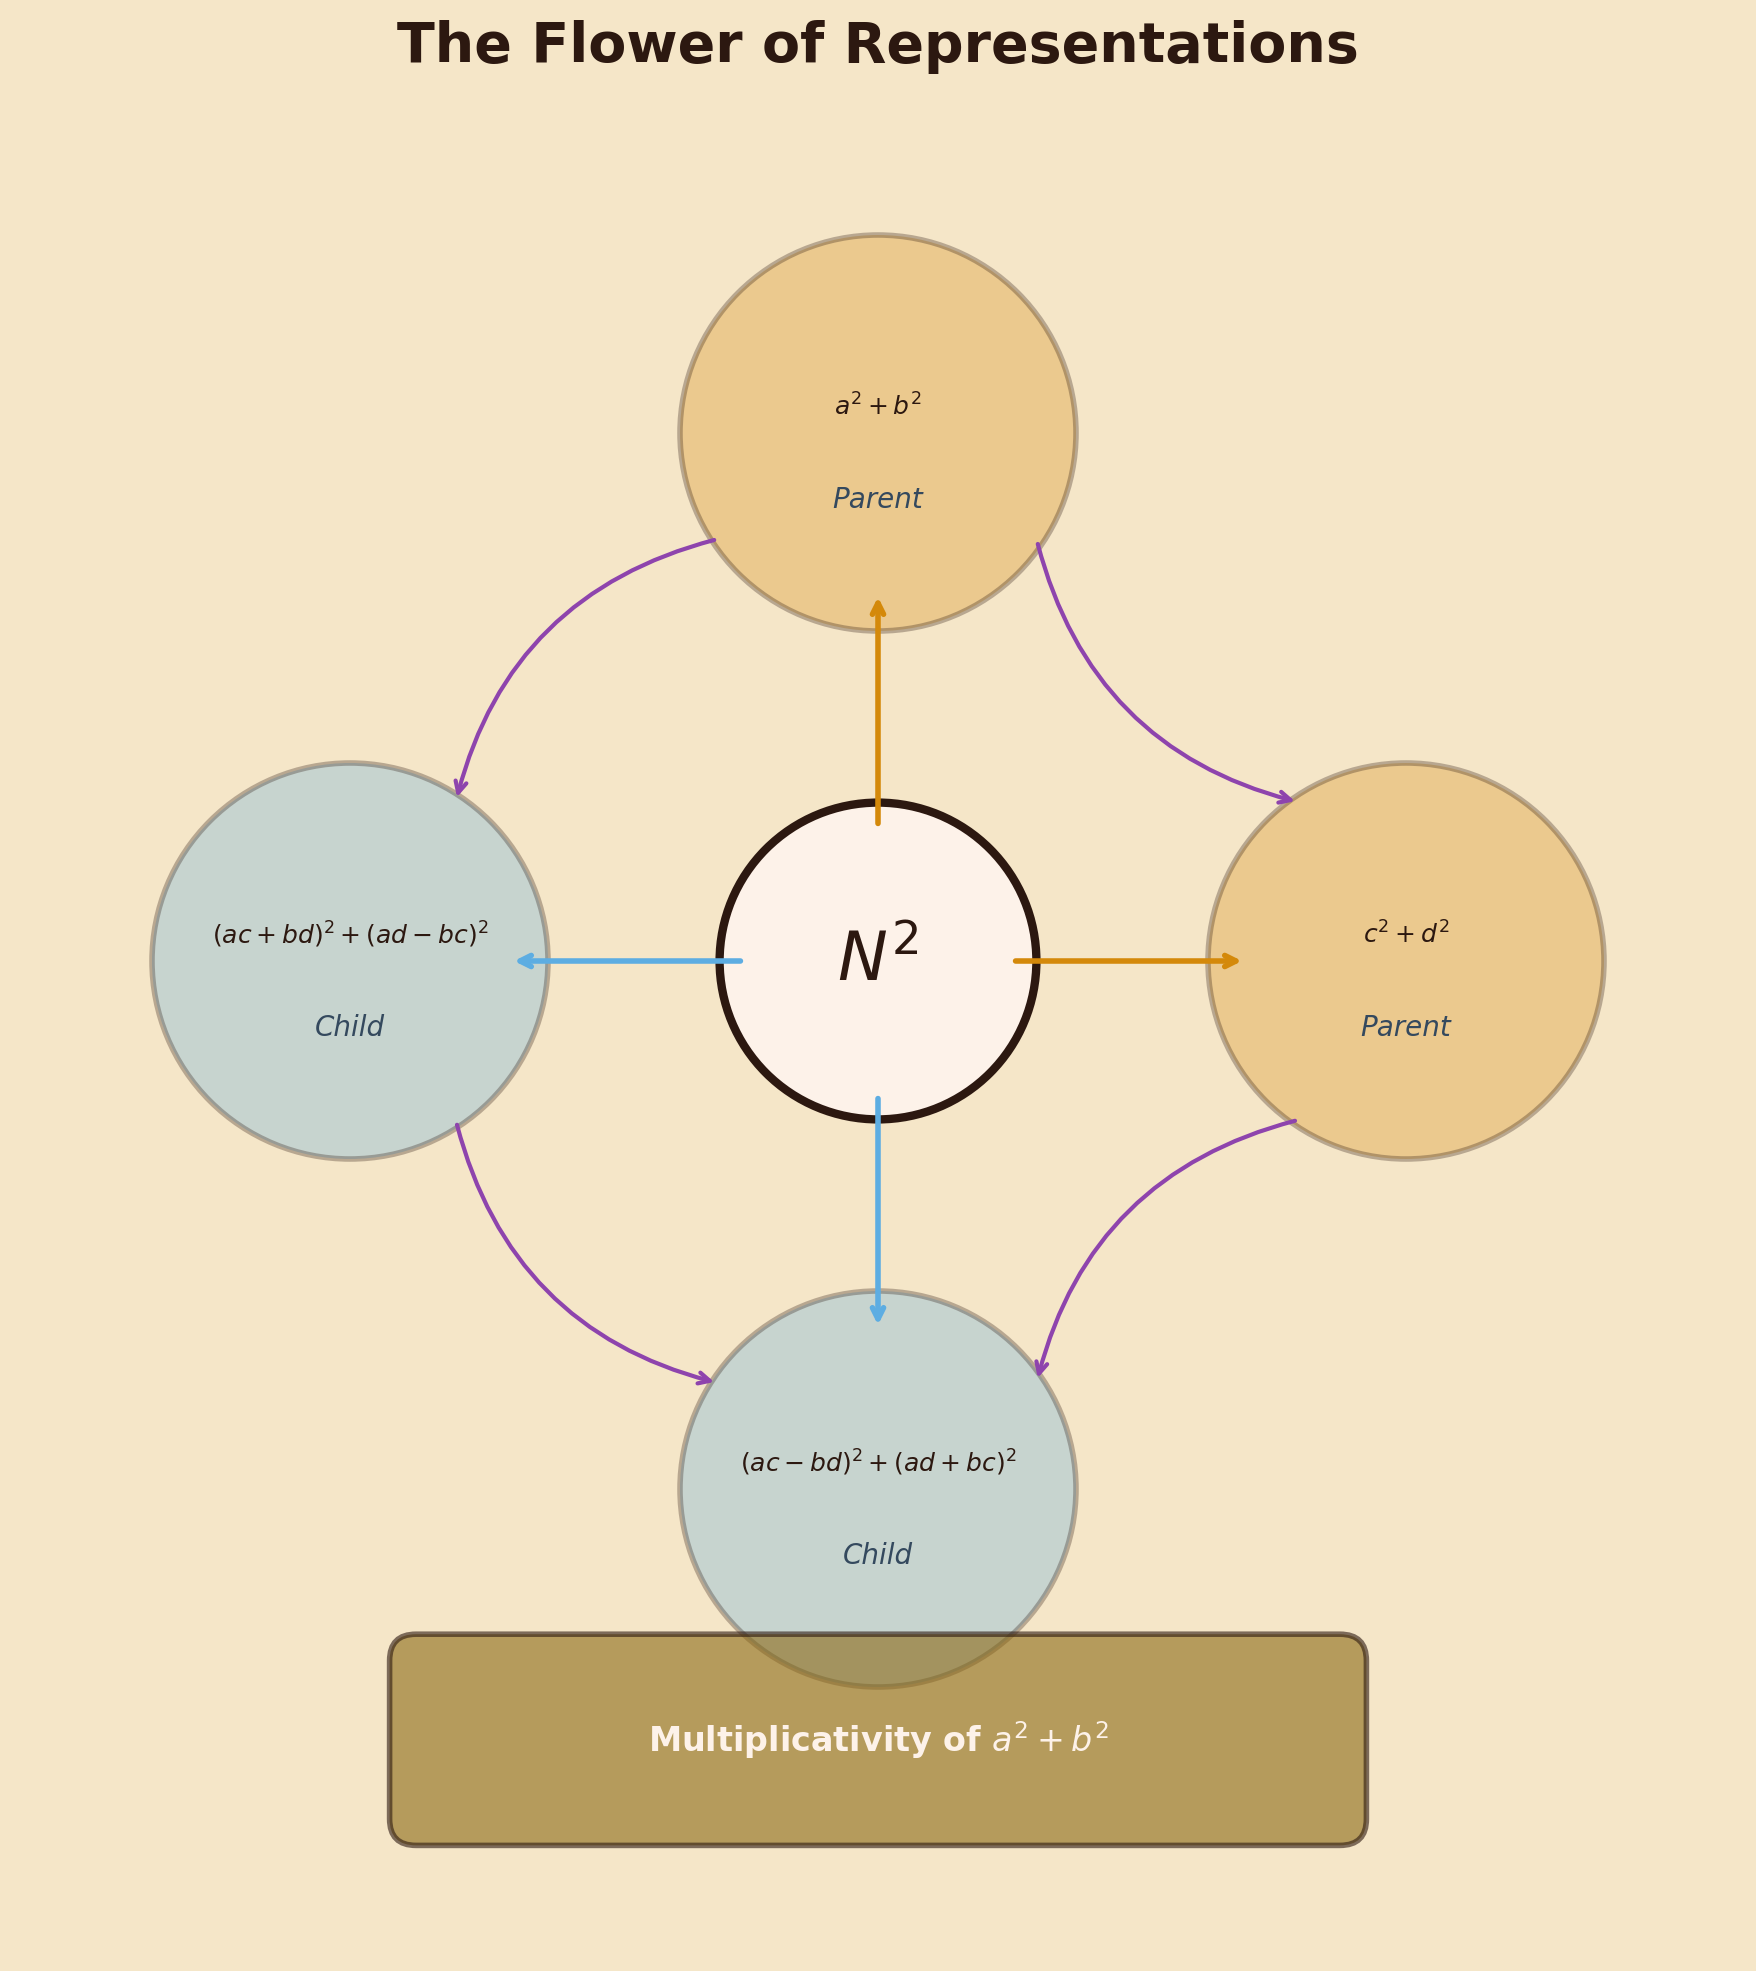
\includegraphics[width=0.85\textwidth]{Chapter4/images/fig14_flower_diagram.png}
\caption{}
\end{figure}
A ``flower'' diagram. At the center, a circle contains \(N^2\). Four petals radiate outward, each containing one sum-of-squares representation of \(N^2\). The top two petals are labeled ``parent representations'' and contain \(a^2 + b^2\) and \(c^2 + d^2\). The bottom two petals are labeled ``children (Brahmagupta--Fibonacci)'' and contain the two composed representations. Curved arrows show which parent pair generates which child. The flower sits in a pot labeled ``Multiplicativity of \(a^2 + b^2\).''{]}

Ramanujan, that incandescent genius, was obsessed with numbers having many representations. His famous taxicab number, \(1729 = 12^3 + 1^3 = 10^3 + 9^3\), is the cubic cousin of our sum-of-squares examples --- the smallest number expressible as a sum of two cubes in two different ways. Hardy called it ``rather a dull number''; Ramanujan saw it was nothing of the kind. The sum-of-squares case is richer still: \(325 = 1^2 + 18^2 = 6^2 + 17^2 = 10^2 + 15^2\) has three representations, and each pair gives Euler a new crack at factoring.

\bigskip\noindent\rule{\linewidth}{0.4pt}\bigskip

\section{The Three Roads Converge --- A Factoring Toolkit}
We have walked all three roads from Pythagoras. Let us stand at the crossroads and survey the complete toolkit.

\begin{longtable}[]{@{}
  >{\raggedright\arraybackslash}p{(\columnwidth - 6\tabcolsep) * \real{0.2500}}
  >{\raggedright\arraybackslash}p{(\columnwidth - 6\tabcolsep) * \real{0.2500}}
  >{\raggedright\arraybackslash}p{(\columnwidth - 6\tabcolsep) * \real{0.2500}}
  >{\raggedright\arraybackslash}p{(\columnwidth - 6\tabcolsep) * \real{0.2500}}@{}}
\toprule\noalign{}
\begin{minipage}[b]{\linewidth}\raggedright
\textbf{Tool}
\end{minipage} & \begin{minipage}[b]{\linewidth}\raggedright
\textbf{Input}
\end{minipage} & \begin{minipage}[b]{\linewidth}\raggedright
\textbf{Output}
\end{minipage} & \begin{minipage}[b]{\linewidth}\raggedright
\textbf{Key Identity}
\end{minipage} \\
\midrule\noalign{}
\endhead
\bottomrule\noalign{}
\endlastfoot
Euler's Method & Two representations \(N = a^2 + b^2 = c^2 + d^2\) & Non-trivial factor of \(N\) & \((a - c)(a + c) = (d - b)(d + b)\) \\
Gaussian Composition & Two Pythagorean triples & New triple with product hypotenuse & \((a_1 a_2 - b_1 b_2)^2 + (a_1 b_2 + b_1 a_2)^2 = (c_1 c_2)^2\) \\
Tree Sieve & Berggren tree + target \(N\) & Smooth relations → factors & \((c - b)(c + b) = N^2\), then \(\gcd\) \\
\end{longtable}

All three methods rest on the same two pillars: the \emph{multiplicativity} of the form \(a^2 + b^2\) (the Brahmagupta--Fibonacci identity) and the \emph{Lorentz invariance} of \(Q = a^2 + b^2 - c^2\) (the Berggren transformations preserve the cone). These two facts --- one algebraic, one geometric --- are the twin engines driving the entire chapter. Every theorem we proved, every trick we demonstrated, is a consequence of one or both.


\begin{figure}[htbp]
\centering
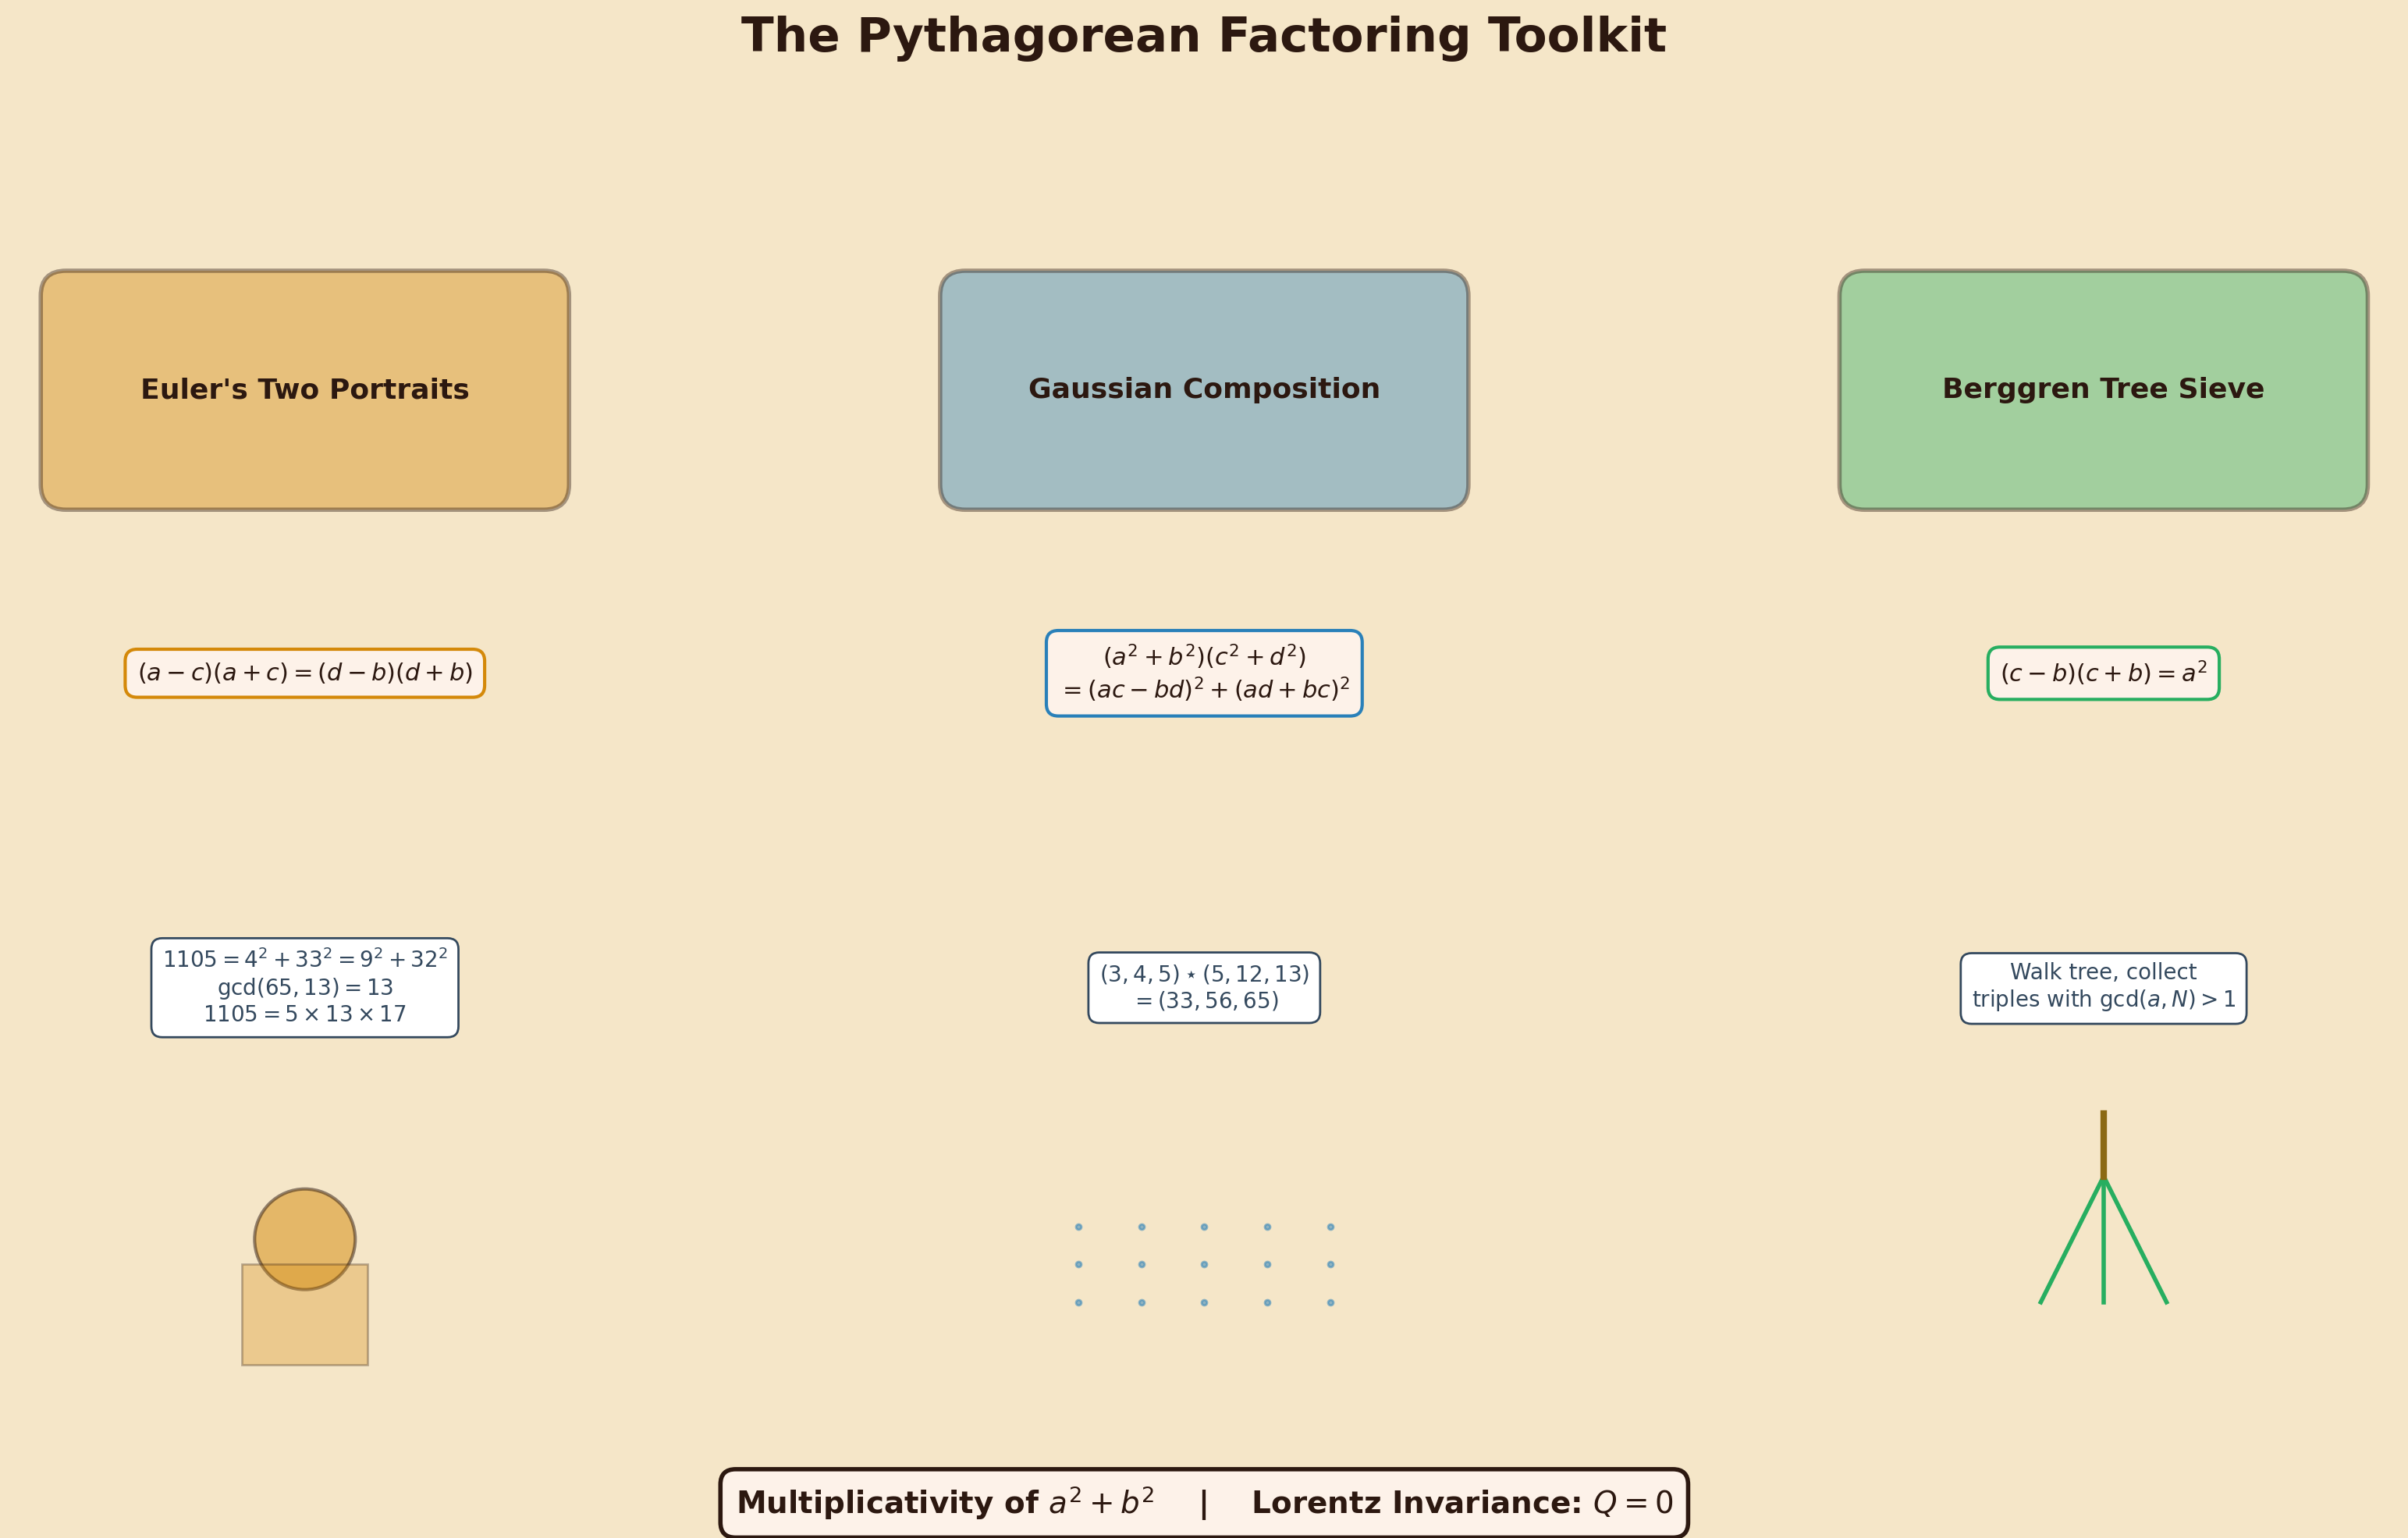
\includegraphics[width=0.85\textwidth]{Chapter4/images/fig15_factoring_toolkit.png}
\caption{}
\end{figure}
A ``Pythagorean Factoring Toolkit'' infographic divided into three columns. Column 1 (amber): ``Euler's Two Portraits'' --- the factoring identity, a worked example with \(N = 1105\), and a small portrait of Euler. Column 2 (blue): ``Gaussian Composition'' --- the Brahmagupta--Fibonacci identity, a worked example with \((3,4,5) \star (5,12,13) = (33,56,65)\), and a small drawing of a Gaussian lattice. Column 3 (green): ``The Berggren Tree Sieve'' --- the divisor equation \((c-b)(c+b) = a^2\), a worked example with the tree, and a small drawing of a branching tree. At the bottom, a shared foundation bar reads: ``Multiplicativity of \(a^2 + b^2\)'' on the left and ``Lorentz Invariance: \(Q = 0\)'' on the right, with both supporting all three columns.{]}

The grand irony is that these methods, beautiful as they are, do not (as far as anyone knows) yield a fast algorithm for factoring large semiprimes. The tree sieve reaches any target in \(\sim \log_3 N\) generations, but finding the right branch requires searching an exponentially large space. Euler's method needs two representations, and finding even one is as hard as factoring itself. Gaussian composition can amplify partial information, but the partial information must come from somewhere.

And yet the ideas in this chapter are not idle curiosities. They are the \emph{ancestors} of the methods that \emph{do} work in practice. The quadratic sieve and the number field sieve --- the fastest known classical factoring algorithms --- are direct descendants of the idea that smooth relations, combined algebraically, can reveal factors. And Shor's quantum algorithm, which would factor large semiprimes in polynomial time on a quantum computer, exploits the same multiplicative structure that Brahmagupta discovered fourteen centuries ago.

In the chapters to come, we will sharpen these tools. We will learn about lattice reduction, which searches the Berggren tree more efficiently by exploiting the geometry of high-dimensional lattices. We will encounter complexity bounds --- precise statements about how many steps the sieve requires --- and discover that the answer scales as \(\Theta(\sqrt{N})\), tantalizingly close to but not quite polynomial. And we will peer into the quantum future, where the interference patterns of qubits accomplish in \(O(N^{1/4})\) steps what classical computers struggle to do at all.


\begin{figure}[htbp]
\centering
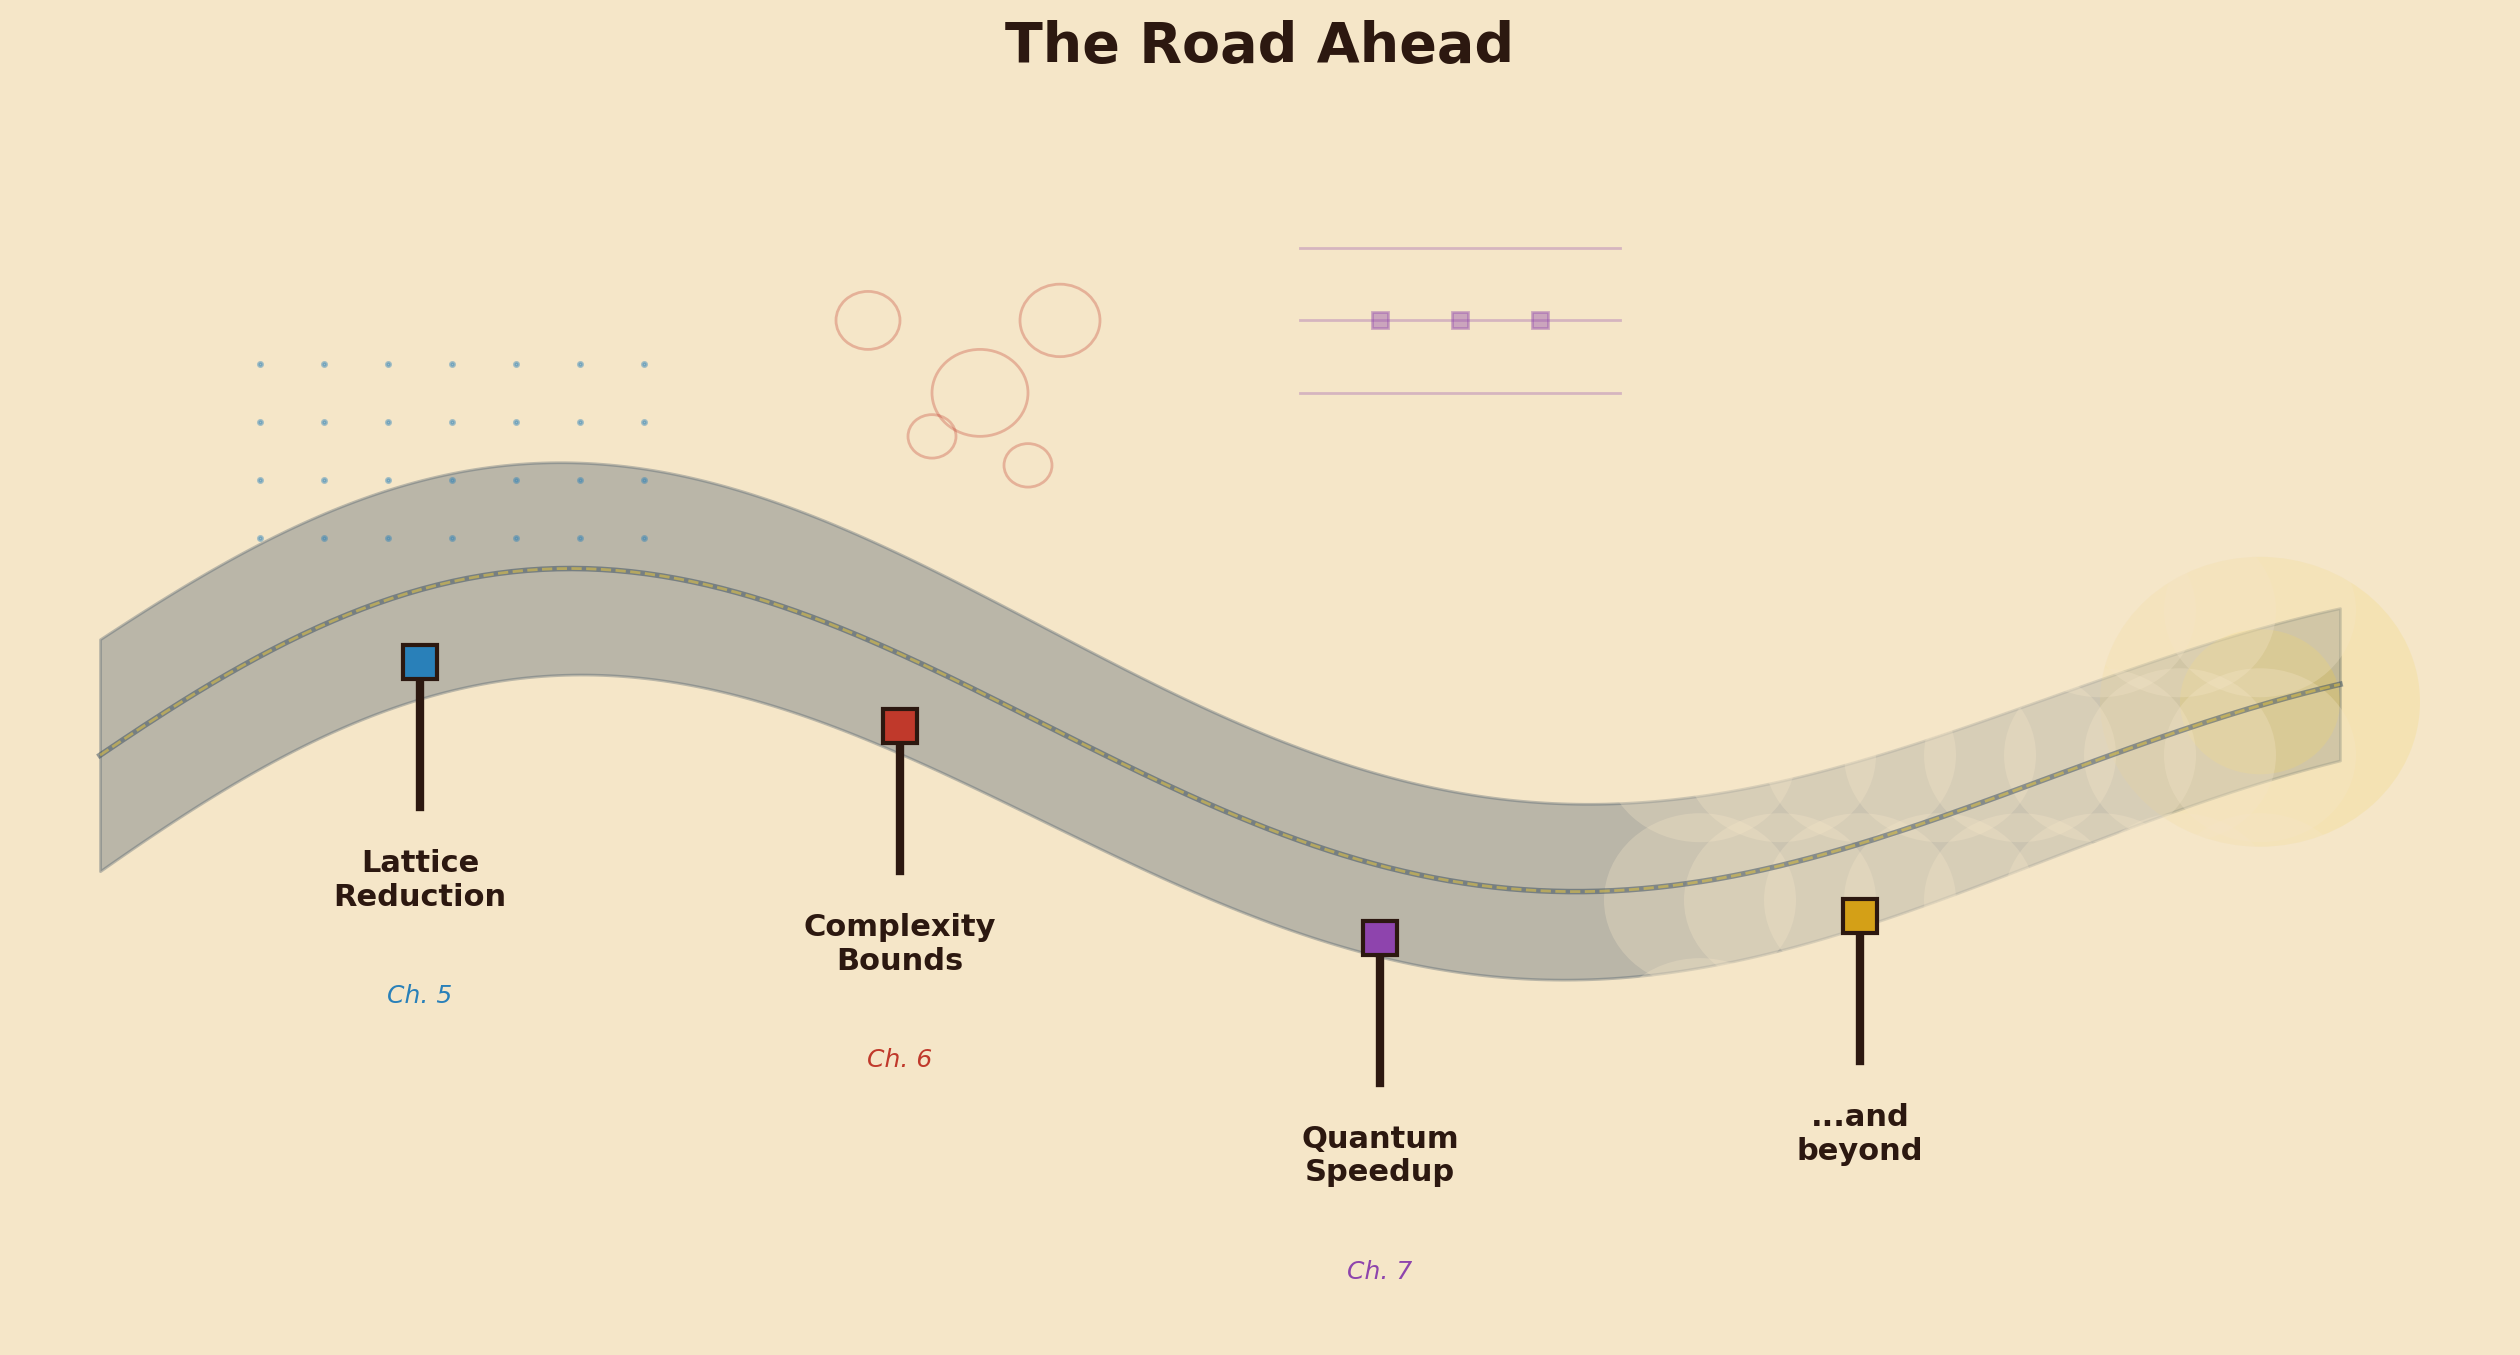
\includegraphics[width=0.85\textwidth]{Chapter4/images/fig16_road_ahead.png}
\caption{}
\end{figure}
A winding road receding into a misty distance. Mile markers along the road are labeled with the topics of future chapters: ``Lattice Reduction'' (Chapter 5), ``Complexity Bounds'' (Chapter 6), ``Quantum Speedup'' (Chapter 7), and beyond. The road passes through varied landscapes --- a field of lattice points, a hyperbolic plane tiling, a shimmering quantum circuit diagram. At the vanishing point, a faint glow suggests something profound waiting to be discovered.{]}

But before you turn the page, here is a parting puzzle to test your mastery of the three roads.

\begin{quote}
\textbf{Closing Puzzle.} The number \(N = 5{,}525\) can be written as a sum of two squares in at least three different ways. Find all three representations, and use Euler's method --- applied to each pair --- to recover the complete prime factorization \(N = 5^2 \times 13 \times 17\).
\end{quote}

\emph{(Hint: Start by noticing that \(5{,}525 = 5 \times 1{,}105\), and recall what we learned about \(1{,}105\) earlier in this chapter\ldots)}

\bigskip\noindent\rule{\linewidth}{0.4pt}\bigskip

\subsection{Puzzles for the Reader}
\begin{quote}
\textbf{Puzzle 1.} Verify the Brahmagupta--Fibonacci identity for \(a = 3\), \(b = 4\), \(c = 5\), \(d = 12\). What two representations of \(5^2 \cdot 13^2 = 4225\) do you obtain?
\end{quote}

\begin{quote}
\textbf{Puzzle 2.} Compose the Pythagorean triples \((8, 15, 17)\) and \((7, 24, 25)\) using the composition theorem. Verify that the result is Pythagorean with hypotenuse \(17 \times 25 = 425\).
\end{quote}

\begin{quote}
\textbf{Puzzle 3.} The number \(901\) can be written as \(1^2 + 30^2\) and as \(10^2 + \sqrt{901 - 100}^2\)\ldots{} but can it? Determine whether \(901\) has two sum-of-squares representations, and if so, use Euler's method to factor it.
\end{quote}

\begin{quote}
\textbf{Puzzle 4.} Apply all three Berggren transformations to \((5, 12, 13)\) and verify that the three children all satisfy \(Q = 0\).
\end{quote}

\begin{quote}
\textbf{Puzzle 5.} Starting from the hypotenuse growth lemma \(c' \geq 3c\), estimate how many generations of the Berggren tree it takes to reach a triple with hypotenuse exceeding one million. Then compute the exact number of nodes you would need to search at that depth.
\end{quote}

\bigskip\noindent\rule{\linewidth}{0.4pt}\bigskip

\emph{The three roads from Pythagoras have shown us how ancient identities can crack modern secrets --- in principle. But ``in principle'' is a long way from ``in practice.'' In the next chapter, we will enter the world of lattices, where geometry and linear algebra join forces to navigate the Berggren tree with something approaching efficiency\ldots{}}
